% Options for packages loaded elsewhere
\PassOptionsToPackage{unicode}{hyperref}
\PassOptionsToPackage{hyphens}{url}
%
\documentclass[
]{article}
\usepackage{lmodern}
\usepackage{amsmath}
\usepackage{ifxetex,ifluatex}
\ifnum 0\ifxetex 1\fi\ifluatex 1\fi=0 % if pdftex
  \usepackage[T1]{fontenc}
  \usepackage[utf8]{inputenc}
  \usepackage{textcomp} % provide euro and other symbols
  \usepackage{amssymb}
\else % if luatex or xetex
  \usepackage{unicode-math}
  \defaultfontfeatures{Scale=MatchLowercase}
  \defaultfontfeatures[\rmfamily]{Ligatures=TeX,Scale=1}
\fi
% Use upquote if available, for straight quotes in verbatim environments
\IfFileExists{upquote.sty}{\usepackage{upquote}}{}
\IfFileExists{microtype.sty}{% use microtype if available
  \usepackage[]{microtype}
  \UseMicrotypeSet[protrusion]{basicmath} % disable protrusion for tt fonts
}{}
\makeatletter
\@ifundefined{KOMAClassName}{% if non-KOMA class
  \IfFileExists{parskip.sty}{%
    \usepackage{parskip}
  }{% else
    \setlength{\parindent}{0pt}
    \setlength{\parskip}{6pt plus 2pt minus 1pt}}
}{% if KOMA class
  \KOMAoptions{parskip=half}}
\makeatother
\usepackage{xcolor}
\IfFileExists{xurl.sty}{\usepackage{xurl}}{} % add URL line breaks if available
\IfFileExists{bookmark.sty}{\usepackage{bookmark}}{\usepackage{hyperref}}
\hypersetup{
  pdftitle={An Introductory Tutorial to Cohort State-Transition Models in R},
  pdfauthor={Fernando Alarid-Escudero, PhD; Eline Krijkamp, MSc; Eva A. Enns, PhD; Alan Yang, MSc; Myriam G.M. Hunink, PhD\^{}\textbackslash dagger; Petros Pechlivanoglou, PhD; Hawre Jalal, MD, PhD},
  pdfkeywords={Markov models, state-transition models, decision models, Tutorial, R},
  hidelinks,
  pdfcreator={LaTeX via pandoc}}
\urlstyle{same} % disable monospaced font for URLs
\usepackage[margin=1in]{geometry}
\usepackage{color}
\usepackage{fancyvrb}
\newcommand{\VerbBar}{|}
\newcommand{\VERB}{\Verb[commandchars=\\\{\}]}
\DefineVerbatimEnvironment{Highlighting}{Verbatim}{commandchars=\\\{\}}
% Add ',fontsize=\small' for more characters per line
\usepackage{framed}
\definecolor{shadecolor}{RGB}{248,248,248}
\newenvironment{Shaded}{\begin{snugshade}}{\end{snugshade}}
\newcommand{\AlertTok}[1]{\textcolor[rgb]{0.94,0.16,0.16}{#1}}
\newcommand{\AnnotationTok}[1]{\textcolor[rgb]{0.56,0.35,0.01}{\textbf{\textit{#1}}}}
\newcommand{\AttributeTok}[1]{\textcolor[rgb]{0.77,0.63,0.00}{#1}}
\newcommand{\BaseNTok}[1]{\textcolor[rgb]{0.00,0.00,0.81}{#1}}
\newcommand{\BuiltInTok}[1]{#1}
\newcommand{\CharTok}[1]{\textcolor[rgb]{0.31,0.60,0.02}{#1}}
\newcommand{\CommentTok}[1]{\textcolor[rgb]{0.56,0.35,0.01}{\textit{#1}}}
\newcommand{\CommentVarTok}[1]{\textcolor[rgb]{0.56,0.35,0.01}{\textbf{\textit{#1}}}}
\newcommand{\ConstantTok}[1]{\textcolor[rgb]{0.00,0.00,0.00}{#1}}
\newcommand{\ControlFlowTok}[1]{\textcolor[rgb]{0.13,0.29,0.53}{\textbf{#1}}}
\newcommand{\DataTypeTok}[1]{\textcolor[rgb]{0.13,0.29,0.53}{#1}}
\newcommand{\DecValTok}[1]{\textcolor[rgb]{0.00,0.00,0.81}{#1}}
\newcommand{\DocumentationTok}[1]{\textcolor[rgb]{0.56,0.35,0.01}{\textbf{\textit{#1}}}}
\newcommand{\ErrorTok}[1]{\textcolor[rgb]{0.64,0.00,0.00}{\textbf{#1}}}
\newcommand{\ExtensionTok}[1]{#1}
\newcommand{\FloatTok}[1]{\textcolor[rgb]{0.00,0.00,0.81}{#1}}
\newcommand{\FunctionTok}[1]{\textcolor[rgb]{0.00,0.00,0.00}{#1}}
\newcommand{\ImportTok}[1]{#1}
\newcommand{\InformationTok}[1]{\textcolor[rgb]{0.56,0.35,0.01}{\textbf{\textit{#1}}}}
\newcommand{\KeywordTok}[1]{\textcolor[rgb]{0.13,0.29,0.53}{\textbf{#1}}}
\newcommand{\NormalTok}[1]{#1}
\newcommand{\OperatorTok}[1]{\textcolor[rgb]{0.81,0.36,0.00}{\textbf{#1}}}
\newcommand{\OtherTok}[1]{\textcolor[rgb]{0.56,0.35,0.01}{#1}}
\newcommand{\PreprocessorTok}[1]{\textcolor[rgb]{0.56,0.35,0.01}{\textit{#1}}}
\newcommand{\RegionMarkerTok}[1]{#1}
\newcommand{\SpecialCharTok}[1]{\textcolor[rgb]{0.00,0.00,0.00}{#1}}
\newcommand{\SpecialStringTok}[1]{\textcolor[rgb]{0.31,0.60,0.02}{#1}}
\newcommand{\StringTok}[1]{\textcolor[rgb]{0.31,0.60,0.02}{#1}}
\newcommand{\VariableTok}[1]{\textcolor[rgb]{0.00,0.00,0.00}{#1}}
\newcommand{\VerbatimStringTok}[1]{\textcolor[rgb]{0.31,0.60,0.02}{#1}}
\newcommand{\WarningTok}[1]{\textcolor[rgb]{0.56,0.35,0.01}{\textbf{\textit{#1}}}}
\usepackage{longtable,booktabs}
\usepackage{calc} % for calculating minipage widths
% Correct order of tables after \paragraph or \subparagraph
\usepackage{etoolbox}
\makeatletter
\patchcmd\longtable{\par}{\if@noskipsec\mbox{}\fi\par}{}{}
\makeatother
% Allow footnotes in longtable head/foot
\IfFileExists{footnotehyper.sty}{\usepackage{footnotehyper}}{\usepackage{footnote}}
\makesavenoteenv{longtable}
\usepackage{graphicx}
\makeatletter
\def\maxwidth{\ifdim\Gin@nat@width>\linewidth\linewidth\else\Gin@nat@width\fi}
\def\maxheight{\ifdim\Gin@nat@height>\textheight\textheight\else\Gin@nat@height\fi}
\makeatother
% Scale images if necessary, so that they will not overflow the page
% margins by default, and it is still possible to overwrite the defaults
% using explicit options in \includegraphics[width, height, ...]{}
\setkeys{Gin}{width=\maxwidth,height=\maxheight,keepaspectratio}
% Set default figure placement to htbp
\makeatletter
\def\fps@figure{htbp}
\makeatother
\setlength{\emergencystretch}{3em} % prevent overfull lines
\providecommand{\tightlist}{%
  \setlength{\itemsep}{0pt}\setlength{\parskip}{0pt}}
\setcounter{secnumdepth}{5}
\usepackage{amsmath}
\usepackage{float}
\usepackage{setspace}\onehalfspacing
\usepackage[printwatermark]{xwatermark}
\newwatermark[allpages,color=gray!20,angle=45,scale=2,xpos=0,ypos=0]{DRAFT, Do Not Share}
\renewcommand{\contentsname}{}\vspace{-.5cm}
\usepackage{booktabs}
\usepackage{longtable}
\usepackage{array}
\usepackage{multirow}
\usepackage{wrapfig}
\usepackage{float}
\usepackage{colortbl}
\usepackage{pdflscape}
\usepackage{tabu}
\usepackage{threeparttable}
\usepackage{threeparttablex}
\usepackage[normalem]{ulem}
\usepackage{makecell}
\usepackage{xcolor}
\ifluatex
  \usepackage{selnolig}  % disable illegal ligatures
\fi
\newlength{\cslhangindent}
\setlength{\cslhangindent}{1.5em}
\newlength{\csllabelwidth}
\setlength{\csllabelwidth}{3em}
\newenvironment{CSLReferences}[2] % #1 hanging-ident, #2 entry spacing
 {% don't indent paragraphs
  \setlength{\parindent}{0pt}
  % turn on hanging indent if param 1 is 1
  \ifodd #1 \everypar{\setlength{\hangindent}{\cslhangindent}}\ignorespaces\fi
  % set entry spacing
  \ifnum #2 > 0
  \setlength{\parskip}{#2\baselineskip}
  \fi
 }%
 {}
\usepackage{calc}
\newcommand{\CSLBlock}[1]{#1\hfill\break}
\newcommand{\CSLLeftMargin}[1]{\parbox[t]{\csllabelwidth}{#1}}
\newcommand{\CSLRightInline}[1]{\parbox[t]{\linewidth - \csllabelwidth}{#1}\break}
\newcommand{\CSLIndent}[1]{\hspace{\cslhangindent}#1}

\title{An Introductory Tutorial to Cohort State-Transition Models in R}
\author{Fernando Alarid-Escudero, PhD\footnote{Division of Public Administration, Center for Research and Teaching in Economics (CIDE), Aguascalientes, AGS, Mexico} \and Eline Krijkamp, MSc\footnote{Department of Epidemiology and Department of Radiology, Erasmus University Medical Center, Rotterdam, The Netherlands} \and Eva A. Enns, PhD\footnote{Division of Health Policy and Management, University of Minnesota School of Public Health, Minneapolis, MN, USA} \and Alan Yang, MSc\footnote{The Hospital for Sick Children, Toronto} \and Myriam G.M. Hunink, PhD\(^\dagger\)\footnote{Center for Health Decision Sciences, Harvard T.H. Chan School of Public Health, Boston, USA} \and Petros Pechlivanoglou, PhD\footnote{The Hospital for Sick Children, Toronto and University of Toronto, Toronto, Ontario, Canada} \and Hawre Jalal, MD, PhD\footnote{University of Pittsburgh, Pittsburgh, PA, USA}}
\date{2021-04-19}

\begin{document}
\maketitle
\begin{abstract}
Decision models can synthesize evidence from different sources to simulate the long-term consequences of alternative strategies in the presence of uncertainty. Cohort state-transition models (cSTM) are decision models commonly used in medical decision-making to simulate hypothetical cohorts' transitions among various health states over time. cSTMs can be time-independent, where transition probabilities are constant over time, or time-dependent, where transition probabilities change over time. This tutorial is the first part of a two-part tutorial on implementing cSTMs in R, an open-source mathematical and statistical programming language. In this tutorial, we implement time-independent cSTMs, while the focus of the accompanying tutorial is on time-dependent cSTM. This tutorial aims to construct time-independent cSTMs using a previously published decision model, calculate costs and effectiveness outcomes, conduct a cost-effectiveness analysis of multiple strategies, and conduct a probabilistic sensitivity analysis. We provide open-source code in R to facilitate wider adoption.
\end{abstract}

{
\setcounter{tocdepth}{2}
\tableofcontents
}
\hypertarget{introduction}{%
\section{Introduction}\label{introduction}}

Policymakers are often tasked with allocating healthcare resources under constrained budgets and uncertainty about future outcomes. Health economic evaluations might inform their final decisions. These economic evaluations often rely on decision models to synthesize evidence from different sources and project long-term outcomes of various alternative strategies. A commonly used decision model is the discrete-time cohort state-transition model (cSTM), often referred to as a Markov model.\textsuperscript{\protect\hyperlink{ref-Kuntz2017}{1}}

In a recent review, we illustrated the increased use of R's statistical programming framework in health decision sciences. We provided a summary of available resources to apply to medical decision making.\textsuperscript{\protect\hyperlink{ref-Jalal2017b}{2}} Many packages have been explicitly developed to estimate and construct cSTMs in R. For example, the \texttt{markovchain}\textsuperscript{\protect\hyperlink{ref-Spedicato2017}{3}} and \texttt{heemod}\textsuperscript{\protect\hyperlink{ref-Filipovic-Pierucci2017}{4}} packages are designed to build cSTMs using a pre-defined structure. The \texttt{markovchain} package focuses on simulating time-independent and time-dependent Markov chains but is not designed to conduct economic evaluations. \texttt{heemod} is a well-structured R package for economic evaluations. Still, it requires users to set up the cSTM structure, specify the parameters, and run analyses in a pre-specified approach, limiting the understanding of how cSTMs work and are constructed. However, these packages are necessarily stylized and inflexible, requiring users to follow a specific cSTM structure. If the desired cSTM does not fit within this structure, using these packages can be challenging.

This tutorial demonstrates how to conduct a full cost-effectiveness analysis (CEA) comparing multiple interventions and implementing probabilistic sensitivity analysis (PSA). We first describe each of the components of a time-independent cSTM. Then, we illustrate the implementation of these components with an example. Our general conceptualization should apply to other programming languages (e.g., MATLAB, Python, C++, Julia). The R code used in this tutorial is provided as supplementary materials so that readers can replicate and modify the example to fit their needs. The reader can find the most up-to-date model code and code to create the tutorial graphs in the accompanying GitHub repository (\url{https://github.com/DARTH-git/cohort-modeling-tutorial-intro}). We assume that the reader is familiar with the basics of decision modeling and has a basic understanding of programming. Thus, a prior introduction to R and linear algebra for decision modelers is recommended.

This introductory tutorial aims to (1) conceptualize time-independent cSTMs for implementation in a programming language and (2) provide a template for implementing these cSTMs in \emph{base} R. We focus on using R \emph{base} packages, ensuring modelers understand the concept and structure of cSTMs and avoid the limitation of constructing cSTMs in a package-specific structure.

\hypertarget{cohort-state-transition-models-cstms}{%
\section{Cohort state-transition models (cSTMs)}\label{cohort-state-transition-models-cstms}}

A cSTM is a dynamic mathematical model in which a hypothetical cohort of individuals transition between different health states over time. In contrast, an individual-based state-transition model (iSTM) is a type of STM where simulated individuals transition between health states over time.\textsuperscript{\protect\hyperlink{ref-Siebert2012c}{5}} We have previously published a tutorial on the implementation of iSTM in R.\textsuperscript{\protect\hyperlink{ref-Krijkamp2018}{6}}

A cSTM is most appropriate when the decision problem has a dynamic component (e.g., the disease process can vary over time) and can be described using a reasonable number of health states. cSTMs are often used because of their transparency, efficiency, ease of development, and debugging. cSTMs are usually computationally less demanding than iSTMs, providing the ability to conduct PSA and value-of-information (VOI) analyses that otherwise might not be computationally feasible with iSTMs.\textsuperscript{\protect\hyperlink{ref-Siebert2012c}{5}} cSTMs have been used to evaluate screening and surveillance programs,\textsuperscript{\protect\hyperlink{ref-Suijkerbuijk2018}{7},\protect\hyperlink{ref-Sathianathen2018a}{8}} diagnostic procedures,\textsuperscript{\protect\hyperlink{ref-Lu2018b}{9}} disease management programs,\textsuperscript{\protect\hyperlink{ref-Djatche2018}{10}}, interventions,\textsuperscript{\protect\hyperlink{ref-Smith-Spangler2010}{11}} and policies.\textsuperscript{\protect\hyperlink{ref-Pershing2014}{12}}

A cSTM consists of a set of \(n_S\) mutually exclusive and collectively exhaustive health states. The cohort is assumed to be homogeneous within each health state. Individuals in the cohort residing in a particular health state are assumed to have the same characteristics and are indistinguishable from one another. The cohort transitions between health states with defined probabilities, which are called ``transition probabilities''. A transition probability represents the chance that individuals in the cohort residing in a state in a given cycle transition to another state or remain in the same state. In cSTMs, a one-cycle transition probability reflects a conditional probability of transitioning during the cycle, given that the person is alive at the beginning of the cycle.\textsuperscript{\protect\hyperlink{ref-Miller1994}{13}}
Transition probabilities only depend on the current health state in a given cycle. They do not depend on the history before that cycle, often referred to as the ``Markovian assumption.''\textsuperscript{\protect\hyperlink{ref-Kuntz2001}{14}--\protect\hyperlink{ref-Beck1983}{16}} This means that in a Markovian cSTM, transition probabilities do not depend on the history of past transitions or time spent in a given state.

cSTMs can be classified as either time-independent (time-homogeneous) or time-dependent (time-inhomogeneous). Time-independent cSTMs have constant transition probabilities (i.e., the probability of any state transition is independent of time). In contrast, time-dependent cSTMs have transition probabilities or other rewards (e.g., costs or utilities associated to being in a particular state ) that vary over time. Time-independent models are simpler to implement than time-dependent ones, but most problems in healthcare are best modeled with time-dependent cSTMs. For example, time-dependent cSTMs can capture the increasing age-specific background mortality as the cohort ages (age dependency) and dependency on the amount of time spent in a given state (state residence dependence). This tutorial focuses on time-independent cSTMs. In the second part tutorial, we describe how to construct time-dependent cSTMs.\textsuperscript{\protect\hyperlink{ref-Alarid-Escudero2021b}{17}}

\hypertarget{rates-versus-probabilities}{%
\subsection{Rates versus probabilities}\label{rates-versus-probabilities}}

Probabilities and rates are commonly used input parameters in cSTMs. While they are often numerically similar in practice, there is a subtle but important conceptual difference. A rate represents the \textit{instantaneous} force of an event occurrence per unit time, while a probability represents the cumulative risk of an event over a defined time period.

To illustrate this difference further, let us assume that after 10,000 person-years of observation of healthy individuals (e.g., 10,000 individuals observed for an average of 1 year, or 5,000 individuals observed for an average of 2 years, etc.), we observe 500 events of interest (e.g., becoming sick from some disease). The annual event rate of becoming sick, \(\mu_{yearly}\), is then equal to \(\mu_{yearly}=500 / 10,000=0.05\).

If we then wanted to know what proportion of an initially healthy cohort becomes sick at the end of the year, we can convert the annual rate of becoming sick into an annual probability of becoming sick using the following relationship:
\begin{equation}
    p_{yearly} = 1-\exp{\left(-\mu_{yearly} \right)}.
    \label{eq:rate-to-prob-ann}
\end{equation}

This equation assumes that the rate of becoming sick is constant over the year, implying that the time until a healthy person becomes sick is exponentially distributed. The parameter \(p_{yearly}\) is the transition probability from healthy to sick in a cSTM when using an annual cycle length.

If we were concerned that an annual cycle length was too long to capture disease dynamics accurately, we could use a monthly cycle length. This would require us to parameterize the model with monthly transition probabilities. To convert the annual probability of becoming sick to a monthly probability, we first calculate the monthly rate of becoming sick:
\begin{equation}
    \mu_{yearly} = -\ln{\left(1-p_{yearly}\right)}.
    \label{eq:prob-to-rate-ann}
\end{equation}

Because rates are instantaneous, the monthly rate is then just the annual rate divided by 12:
\begin{equation}
    \mu_{monthly} = \mu_{yearly} / 12.
    \label{eq:rate-ann-to-month}
\end{equation}

We divide by 12 because this is the number of months (desired cycle length) in a year (cycle length of the given data). If the original or desired cycle length were different, we would divide by a different factor (e.g., annual to weekly: 52; annual to daily: 365.25, etc.).

The monthly probability can then be calculated from the monthly rate using equation \eqref{eq:rate-to-prob-ann}:
\begin{equation}
    p_{monthly} = 1-\exp{\left(-\mu_{monthly}\right)}.
    \label{eq:rate-to-prob-month}
\end{equation}

Sometimes, transition probabilities might be available from published literature in one time period (e.g., annual). In contrast, the model cycle length could be in a different time scale (e.g., monthly), requiring the analyst to convert the transition probability to the desired cycle length using the equations described above. Furthermore, the conversion may differ for different parameters if they come from various sources and cycle lengths.

\hypertarget{time-independent-cstm-dynamics}{%
\section{Time-independent cSTM dynamics}\label{time-independent-cstm-dynamics}}

A cSTM consists of three core components: (1) a state vector, \(\mathbf{m}_t\), that stores the distribution of the cohort across all health states in cycle \(t\) where \(t = 0,\ldots, n_T\); (2) the cohort trace matrix, \(M\), that stacks \(\mathbf{m}_t\) for all \(t\) and represents the distribution of the cohort in the various states over time; and (3) a transition probability matrix, \(P\).\textsuperscript{\protect\hyperlink{ref-Iskandar2018a}{18}} If the cSTM is comprised of \(n_S\) discrete health states, \(\mathbf{m}_t\) is a \(1 \times n_S\) vector and \(P\) is a \(n_S \times n_S\) matrix. The \(i\)-th element of \(\mathbf{m}_t\), where \(i = 1,\ldots, n_S\), represents the proportion of the cohort in the \(i\)-th health state in cycle \(t\), referred to as \(m_{[t,i]}\). Thus, \(\mathbf{m}_t\) is written as:
\[
\mathbf{m}_t =
  \begin{bmatrix}
m_{[t,1]} & m_{[t,2]} & \cdots & m_{[t,n_S]}
\end{bmatrix}.
\]
The elements of \(P\) are the transition probabilities of moving from state \(i\) to state \(j\), \(p_{[i,j]}\), where \(\{i,j\} = 1,\ldots, n_S\) and all should have values between 0 and 1.
\[
  P = 
  \begin{bmatrix}
    p_{[1,1]} & p_{[1,2]} & \cdots & p_{[1,n_S]} \\
    p_{[2,1]} & p_{[2,2]} & \cdots & p_{[2,n_S]} \\
    \vdots    & \vdots  & \ddots & \vdots   \\
    p_{[n_S,1]} & p_{[n_S,2]} & \cdots & p_{[n_S,n_S]} \\
  \end{bmatrix}.
\]
For \(P\) to be a correctly specified transition probability matrix, all rows of the transition probability matrix must sum to one, \(\sum_{j=1}^{n_S}{p_{[i,j]}} = 1\) for all \(i = 1,\ldots,n_S\).

The state vector at cycle \(t+1\) (\(\mathbf{m}_{t+1}\)) is then calculated as the matrix product of the state vector at cycle \(t\), \(\mathbf{m}_{t}\), and the transition probability matrix, \(P\), such that

\[
  \mathbf{m}_{t+1} = \mathbf{m}_{t} P \text{ for } t = 0,\ldots, (n_T - 1),
\]
where \(\mathbf{m}_1\) is computed from \(\mathbf{m}_{0}\), the initial state vector with the distribution of the cohort across all health states at the start of the simulation (cycle 0). Then, we iteratively apply this equation through \(t = \left(n_T-1 \right)\).

The cohort trace matrix, \(M\), is a matrix of dimensions \((n_T+1) \times n_S\) where each row is a state vector \((-\mathbf{m}_{t}-)\), such that

\[
  M = 
  \begin{bmatrix}
    - \mathbf{m}_0 -  \\
    - \mathbf{m}_1 -  \\
     \vdots \\
    - \mathbf{m}_{n_T} -  
  \end{bmatrix}. 
\]

Note that the initial cycle (i.e., cycle 0) corresponds to \(t=0\), which is on the first row of \(M\). Thus, \(M\) stores the output of the cSTM, which could be used to compute various epidemiological, and economic outcomes, such as life expectancy, prevalence, cumulative resource use, and costs, etc. Table \ref{tab:cSTM-components-table} describes the elements related to the core components of cSTM and their suggested R code names. For a more detailed description of the variable types, data structure, R name for all cSTM elements, please see the Supplementary Material.

\begin{longtable}[]{@{}llcl@{}}
\caption{\label{tab:cSTM-components-table} Components of a cSTM with their R name.}\tabularnewline
\toprule
Element & Description & R name &\tabularnewline
\midrule
\endfirsthead
\toprule
Element & Description & R name &\tabularnewline
\midrule
\endhead
\(n_S\) & Number of states & \texttt{n\_states} &\tabularnewline
\(\mathbf{m}_0\) & Initial state vector & \texttt{v\_m\_init} &\tabularnewline
\(\mathbf{m}_t\) & State vector in cycle \(t\) & \texttt{v\_mt} &\tabularnewline
\(M\) & Cohort trace matrix & \texttt{m\_M} &\tabularnewline
\(P\) & Time-independent transition probability matrix & \texttt{m\_P} &\tabularnewline
\bottomrule
\end{longtable}

\hypertarget{case-study-sick-sicker-model}{%
\section{Case study: Sick-Sicker model}\label{case-study-sick-sicker-model}}

In this tutorial, we will use the previously published 4-state ``Sick-Sicker'' model for conducting a cost-effectiveness analysis (CEA) of multiple strategies to illustrate the various aspects of cSTM implementation in R.\textsuperscript{\protect\hyperlink{ref-Krijkamp2018}{6},\protect\hyperlink{ref-Enns2015e}{19}} Figure \ref{fig:STD-Sick-Sicker} represents the state-transition diagram of the Sick-Sicker model.

\begin{figure}[H]

{\centering 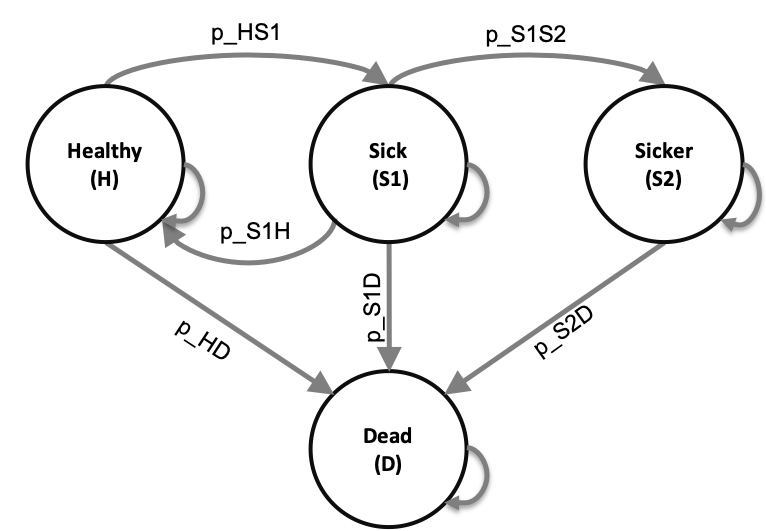
\includegraphics[width=10.64in]{figs/Sick-Sicker} 

}

\caption{State-transition diagram of the time-independent Sick-Sicker cohort state-transition model, showing all possible states (labeled with state names) and transitions (labeled with transition probability variable names).}\label{fig:STD-Sick-Sicker}
\end{figure}

The model simulates a cohort at risk of a hypothetical disease with two stages, ``Sick'' and ``Sicker'', to compute the expected costs and quality-adjusted life years (QALYs) of the cohort over time.
All the parameters of the Sick-Sicker model and the corresponding R variable names are presented in Table \ref{tab:param-table}. The naming of these parameters and variables follows the notation described in the DARTH coding framework.\textsuperscript{\protect\hyperlink{ref-Alarid-Escudero2019e}{20}} Briefly, we define variables by \texttt{\textless{}x\textgreater{}\_\textless{}y\textgreater{}\_\textless{}var\_name\textgreater{}}, where \texttt{x} is the prefix that indicates the data type (e.g., scalar (no prefix), \texttt{v} for vector, \texttt{m} for matrix, \texttt{a} for array, \texttt{df} for data frame, etc.), \texttt{y} is the prefix indicating variable type (e.g., \texttt{p} for probability, \texttt{r} for rate, \texttt{hr} for hazard ratio, \texttt{lor} for log-odds ratio, \texttt{c} for cost \texttt{c}, \texttt{u}for utility, etc.), and \texttt{var\_name} is some description of the variable presented separated by underscores. For example, \texttt{v\_p\_HD} denotes the vector of transition probabilities from health state ``H'' to health state ``D''. In later sections we will define and name all the other parameters.

In the Sick-Sicker model, we simulate a hypothetical cohort of 25-year-old individuals over their lifetime (until to a maximum age of 100 years) who all start in the ``Healthy'' state (denoted ``H''). We will simulate the cohort dynamics in annual cycle lengths, requiring a total of 75 one-year cycles. The total number of cycles is denoted as \(n_T\) and defined in R as \texttt{n\_cycles}. Healthy individuals are at risk of developing the disease when they transition to the ``Sick'' state (denoted by ``S1''). Sick individuals are at risk of further progressing to a more severe disease stage, the ``Sicker'' health state (denoted by ``S2''). Individuals in S1 can recover and return to H. However, once individuals reach S2, they cannot recover; that is, the probability of transitioning to S1 or H from S2 is zero. Individuals in H face constant background mortality. Individuals in S1 and S2 face an increased hazard of death, compared to healthy individuals, in the form of a hazard ratio (HR) of 3 and 10, respectively, relative to the background mortality rate. Individuals in S1 and S2 also experience increased health care costs, and reduced quality of life (QoL) compared to individuals in H. When individuals die, they transition to the absorbing ``Dead'' state (denoted by ``D''), where they remain. All transitions between non-death states are assumed to be conditional on surviving each cycle. We discount both costs and QALYs at an annual rate of 3\%.

We are interested in evaluating the cost-effectiveness of four strategies: the standard of care (strategy SoC), strategy A, strategy B, and a combination of strategies A and B (strategy AB). Strategy A involves administering treatment A that increases the QoL of individuals in S1 from 0.75 (utility without treatment, \texttt{u\_S1}) to 0.95 (utility with treatment A, \texttt{u\_trtA}) and costs \$12,000 per year (\texttt{c\_trtA}).\textsuperscript{\protect\hyperlink{ref-Krijkamp2018}{6}} This strategy does not impact the QoL of individuals in S2, nor does it change the risk of becoming sick or progressing through the sick states. Strategy B uses treatment B to reduce only the rate of Sick individuals progressing to the Sicker state with a hazard ratio (HR) of 0.6 (\texttt{hr\_S1S2\_trtB}), costs \$13,000 per year (\texttt{c\_trtB}), and does not affect QoL. Strategy AB involves administering both treatments A and B.

We assume that it is not possible to distinguish between Sick and Sicker patients; therefore, for treatment strategies, individuals in both disease states receive the treatment. After comparing the four strategies in terms of expected QALYs and costs, we calculate the incremental cost per QALY gained between non-dominated strategies.

\begin{longtable}[]{@{}lccc@{}}
\caption{\label{tab:param-table} Description of parameters, their R variable name, base-case values and distribution.}\tabularnewline
\toprule
\begin{minipage}[b]{(\columnwidth - 3\tabcolsep) * \real{0.45}}\raggedright
\textbf{Parameter}\strut
\end{minipage} & \begin{minipage}[b]{(\columnwidth - 3\tabcolsep) * \real{0.16}}\centering
\textbf{R name}\strut
\end{minipage} & \begin{minipage}[b]{(\columnwidth - 3\tabcolsep) * \real{0.19}}\centering
\textbf{Base-case}\strut
\end{minipage} & \begin{minipage}[b]{(\columnwidth - 3\tabcolsep) * \real{0.20}}\centering
\textbf{Distribution}\strut
\end{minipage}\tabularnewline
\midrule
\endfirsthead
\toprule
\begin{minipage}[b]{(\columnwidth - 3\tabcolsep) * \real{0.45}}\raggedright
\textbf{Parameter}\strut
\end{minipage} & \begin{minipage}[b]{(\columnwidth - 3\tabcolsep) * \real{0.16}}\centering
\textbf{R name}\strut
\end{minipage} & \begin{minipage}[b]{(\columnwidth - 3\tabcolsep) * \real{0.19}}\centering
\textbf{Base-case}\strut
\end{minipage} & \begin{minipage}[b]{(\columnwidth - 3\tabcolsep) * \real{0.20}}\centering
\textbf{Distribution}\strut
\end{minipage}\tabularnewline
\midrule
\endhead
\begin{minipage}[t]{(\columnwidth - 3\tabcolsep) * \real{0.45}}\raggedright
Number of cycles (\(n_cycles\))\strut
\end{minipage} & \begin{minipage}[t]{(\columnwidth - 3\tabcolsep) * \real{0.16}}\centering
\texttt{n\_cycles}\strut
\end{minipage} & \begin{minipage}[t]{(\columnwidth - 3\tabcolsep) * \real{0.19}}\centering
75 years\strut
\end{minipage} & \begin{minipage}[t]{(\columnwidth - 3\tabcolsep) * \real{0.20}}\centering
-\strut
\end{minipage}\tabularnewline
\begin{minipage}[t]{(\columnwidth - 3\tabcolsep) * \real{0.45}}\raggedright
Names of health states (\(n\))\strut
\end{minipage} & \begin{minipage}[t]{(\columnwidth - 3\tabcolsep) * \real{0.16}}\centering
\texttt{v\_names\_states}\strut
\end{minipage} & \begin{minipage}[t]{(\columnwidth - 3\tabcolsep) * \real{0.19}}\centering
H, S1, S2, D\strut
\end{minipage} & \begin{minipage}[t]{(\columnwidth - 3\tabcolsep) * \real{0.20}}\centering
-\strut
\end{minipage}\tabularnewline
\begin{minipage}[t]{(\columnwidth - 3\tabcolsep) * \real{0.45}}\raggedright
Annual discount rate for costs\strut
\end{minipage} & \begin{minipage}[t]{(\columnwidth - 3\tabcolsep) * \real{0.16}}\centering
\texttt{d\_c}\strut
\end{minipage} & \begin{minipage}[t]{(\columnwidth - 3\tabcolsep) * \real{0.19}}\centering
3\%\strut
\end{minipage} & \begin{minipage}[t]{(\columnwidth - 3\tabcolsep) * \real{0.20}}\centering
-\strut
\end{minipage}\tabularnewline
\begin{minipage}[t]{(\columnwidth - 3\tabcolsep) * \real{0.45}}\raggedright
Annual discount rate for QALYs\strut
\end{minipage} & \begin{minipage}[t]{(\columnwidth - 3\tabcolsep) * \real{0.16}}\centering
\texttt{d\_e}\strut
\end{minipage} & \begin{minipage}[t]{(\columnwidth - 3\tabcolsep) * \real{0.19}}\centering
3\%\strut
\end{minipage} & \begin{minipage}[t]{(\columnwidth - 3\tabcolsep) * \real{0.20}}\centering
-\strut
\end{minipage}\tabularnewline
\begin{minipage}[t]{(\columnwidth - 3\tabcolsep) * \real{0.45}}\raggedright
Number of PSA samples (\(K\))\strut
\end{minipage} & \begin{minipage}[t]{(\columnwidth - 3\tabcolsep) * \real{0.16}}\centering
\texttt{n\_sim}\strut
\end{minipage} & \begin{minipage}[t]{(\columnwidth - 3\tabcolsep) * \real{0.19}}\centering
1,000\strut
\end{minipage} & \begin{minipage}[t]{(\columnwidth - 3\tabcolsep) * \real{0.20}}\centering
-\strut
\end{minipage}\tabularnewline
\begin{minipage}[t]{(\columnwidth - 3\tabcolsep) * \real{0.45}}\raggedright
Annual transition probabilities conditional on surviving\strut
\end{minipage} & \begin{minipage}[t]{(\columnwidth - 3\tabcolsep) * \real{0.16}}\centering
\strut
\end{minipage} & \begin{minipage}[t]{(\columnwidth - 3\tabcolsep) * \real{0.19}}\centering
\strut
\end{minipage} & \begin{minipage}[t]{(\columnwidth - 3\tabcolsep) * \real{0.20}}\centering
\strut
\end{minipage}\tabularnewline
\begin{minipage}[t]{(\columnwidth - 3\tabcolsep) * \real{0.45}}\raggedright
- Disease onset (H to S1)\strut
\end{minipage} & \begin{minipage}[t]{(\columnwidth - 3\tabcolsep) * \real{0.16}}\centering
\texttt{p\_HS1}\strut
\end{minipage} & \begin{minipage}[t]{(\columnwidth - 3\tabcolsep) * \real{0.19}}\centering
0.150\strut
\end{minipage} & \begin{minipage}[t]{(\columnwidth - 3\tabcolsep) * \real{0.20}}\centering
beta(30, 170)\strut
\end{minipage}\tabularnewline
\begin{minipage}[t]{(\columnwidth - 3\tabcolsep) * \real{0.45}}\raggedright
- Recovery (S1 to H)\strut
\end{minipage} & \begin{minipage}[t]{(\columnwidth - 3\tabcolsep) * \real{0.16}}\centering
\texttt{p\_S1H}\strut
\end{minipage} & \begin{minipage}[t]{(\columnwidth - 3\tabcolsep) * \real{0.19}}\centering
0.500\strut
\end{minipage} & \begin{minipage}[t]{(\columnwidth - 3\tabcolsep) * \real{0.20}}\centering
beta(60, 60)\strut
\end{minipage}\tabularnewline
\begin{minipage}[t]{(\columnwidth - 3\tabcolsep) * \real{0.45}}\raggedright
- Disease progression (S1 to S2)\strut
\end{minipage} & \begin{minipage}[t]{(\columnwidth - 3\tabcolsep) * \real{0.16}}\centering
\texttt{p\_S1S2}\strut
\end{minipage} & \begin{minipage}[t]{(\columnwidth - 3\tabcolsep) * \real{0.19}}\centering
0.105\strut
\end{minipage} & \begin{minipage}[t]{(\columnwidth - 3\tabcolsep) * \real{0.20}}\centering
beta(84, 716)\strut
\end{minipage}\tabularnewline
\begin{minipage}[t]{(\columnwidth - 3\tabcolsep) * \real{0.45}}\raggedright
Annual mortality\strut
\end{minipage} & \begin{minipage}[t]{(\columnwidth - 3\tabcolsep) * \real{0.16}}\centering
\strut
\end{minipage} & \begin{minipage}[t]{(\columnwidth - 3\tabcolsep) * \real{0.19}}\centering
\strut
\end{minipage} & \begin{minipage}[t]{(\columnwidth - 3\tabcolsep) * \real{0.20}}\centering
\strut
\end{minipage}\tabularnewline
\begin{minipage}[t]{(\columnwidth - 3\tabcolsep) * \real{0.45}}\raggedright
- Background mortality rate (H to D)\strut
\end{minipage} & \begin{minipage}[t]{(\columnwidth - 3\tabcolsep) * \real{0.16}}\centering
\texttt{r\_HD}\strut
\end{minipage} & \begin{minipage}[t]{(\columnwidth - 3\tabcolsep) * \real{0.19}}\centering
0.002\strut
\end{minipage} & \begin{minipage}[t]{(\columnwidth - 3\tabcolsep) * \real{0.20}}\centering
-\strut
\end{minipage}\tabularnewline
\begin{minipage}[t]{(\columnwidth - 3\tabcolsep) * \real{0.45}}\raggedright
- Hazard ratio of death in S1 vs H\strut
\end{minipage} & \begin{minipage}[t]{(\columnwidth - 3\tabcolsep) * \real{0.16}}\centering
\texttt{hr\_S1}\strut
\end{minipage} & \begin{minipage}[t]{(\columnwidth - 3\tabcolsep) * \real{0.19}}\centering
3.0\strut
\end{minipage} & \begin{minipage}[t]{(\columnwidth - 3\tabcolsep) * \real{0.20}}\centering
lognormal(log(3.0), 0.01)\strut
\end{minipage}\tabularnewline
\begin{minipage}[t]{(\columnwidth - 3\tabcolsep) * \real{0.45}}\raggedright
- Hazard ratio of death in S2 vs H\strut
\end{minipage} & \begin{minipage}[t]{(\columnwidth - 3\tabcolsep) * \real{0.16}}\centering
\texttt{hr\_S2}\strut
\end{minipage} & \begin{minipage}[t]{(\columnwidth - 3\tabcolsep) * \real{0.19}}\centering
10.0\strut
\end{minipage} & \begin{minipage}[t]{(\columnwidth - 3\tabcolsep) * \real{0.20}}\centering
lognormal(log(10.0), 0.02)\strut
\end{minipage}\tabularnewline
\begin{minipage}[t]{(\columnwidth - 3\tabcolsep) * \real{0.45}}\raggedright
Annual costs\strut
\end{minipage} & \begin{minipage}[t]{(\columnwidth - 3\tabcolsep) * \real{0.16}}\centering
\strut
\end{minipage} & \begin{minipage}[t]{(\columnwidth - 3\tabcolsep) * \real{0.19}}\centering
\strut
\end{minipage} & \begin{minipage}[t]{(\columnwidth - 3\tabcolsep) * \real{0.20}}\centering
\strut
\end{minipage}\tabularnewline
\begin{minipage}[t]{(\columnwidth - 3\tabcolsep) * \real{0.45}}\raggedright
- Healthy individuals\strut
\end{minipage} & \begin{minipage}[t]{(\columnwidth - 3\tabcolsep) * \real{0.16}}\centering
\texttt{c\_H}\strut
\end{minipage} & \begin{minipage}[t]{(\columnwidth - 3\tabcolsep) * \real{0.19}}\centering
\$2,000\strut
\end{minipage} & \begin{minipage}[t]{(\columnwidth - 3\tabcolsep) * \real{0.20}}\centering
gamma(100.0, 20.0)\strut
\end{minipage}\tabularnewline
\begin{minipage}[t]{(\columnwidth - 3\tabcolsep) * \real{0.45}}\raggedright
- Sick individuals in S1\strut
\end{minipage} & \begin{minipage}[t]{(\columnwidth - 3\tabcolsep) * \real{0.16}}\centering
\texttt{c\_S1}\strut
\end{minipage} & \begin{minipage}[t]{(\columnwidth - 3\tabcolsep) * \real{0.19}}\centering
\$4,000\strut
\end{minipage} & \begin{minipage}[t]{(\columnwidth - 3\tabcolsep) * \real{0.20}}\centering
gamma(177.8, 22.5)\strut
\end{minipage}\tabularnewline
\begin{minipage}[t]{(\columnwidth - 3\tabcolsep) * \real{0.45}}\raggedright
- Sick individuals in S2\strut
\end{minipage} & \begin{minipage}[t]{(\columnwidth - 3\tabcolsep) * \real{0.16}}\centering
\texttt{c\_S2}\strut
\end{minipage} & \begin{minipage}[t]{(\columnwidth - 3\tabcolsep) * \real{0.19}}\centering
\$15,000\strut
\end{minipage} & \begin{minipage}[t]{(\columnwidth - 3\tabcolsep) * \real{0.20}}\centering
gamma(225.0, 66.7)\strut
\end{minipage}\tabularnewline
\begin{minipage}[t]{(\columnwidth - 3\tabcolsep) * \real{0.45}}\raggedright
- Dead individuals\strut
\end{minipage} & \begin{minipage}[t]{(\columnwidth - 3\tabcolsep) * \real{0.16}}\centering
\texttt{c\_D}\strut
\end{minipage} & \begin{minipage}[t]{(\columnwidth - 3\tabcolsep) * \real{0.19}}\centering
\$0\strut
\end{minipage} & \begin{minipage}[t]{(\columnwidth - 3\tabcolsep) * \real{0.20}}\centering
-\strut
\end{minipage}\tabularnewline
\begin{minipage}[t]{(\columnwidth - 3\tabcolsep) * \real{0.45}}\raggedright
Utility weights\strut
\end{minipage} & \begin{minipage}[t]{(\columnwidth - 3\tabcolsep) * \real{0.16}}\centering
\strut
\end{minipage} & \begin{minipage}[t]{(\columnwidth - 3\tabcolsep) * \real{0.19}}\centering
\strut
\end{minipage} & \begin{minipage}[t]{(\columnwidth - 3\tabcolsep) * \real{0.20}}\centering
\strut
\end{minipage}\tabularnewline
\begin{minipage}[t]{(\columnwidth - 3\tabcolsep) * \real{0.45}}\raggedright
- Healthy individuals\strut
\end{minipage} & \begin{minipage}[t]{(\columnwidth - 3\tabcolsep) * \real{0.16}}\centering
\texttt{u\_H}\strut
\end{minipage} & \begin{minipage}[t]{(\columnwidth - 3\tabcolsep) * \real{0.19}}\centering
1.00\strut
\end{minipage} & \begin{minipage}[t]{(\columnwidth - 3\tabcolsep) * \real{0.20}}\centering
beta(200, 3)\strut
\end{minipage}\tabularnewline
\begin{minipage}[t]{(\columnwidth - 3\tabcolsep) * \real{0.45}}\raggedright
- Sick individuals in S1\strut
\end{minipage} & \begin{minipage}[t]{(\columnwidth - 3\tabcolsep) * \real{0.16}}\centering
\texttt{u\_S1}\strut
\end{minipage} & \begin{minipage}[t]{(\columnwidth - 3\tabcolsep) * \real{0.19}}\centering
0.75\strut
\end{minipage} & \begin{minipage}[t]{(\columnwidth - 3\tabcolsep) * \real{0.20}}\centering
beta(130, 45)\strut
\end{minipage}\tabularnewline
\begin{minipage}[t]{(\columnwidth - 3\tabcolsep) * \real{0.45}}\raggedright
- Sick individuals in S2\strut
\end{minipage} & \begin{minipage}[t]{(\columnwidth - 3\tabcolsep) * \real{0.16}}\centering
\texttt{u\_S2}\strut
\end{minipage} & \begin{minipage}[t]{(\columnwidth - 3\tabcolsep) * \real{0.19}}\centering
0.50\strut
\end{minipage} & \begin{minipage}[t]{(\columnwidth - 3\tabcolsep) * \real{0.20}}\centering
beta(230, 230)\strut
\end{minipage}\tabularnewline
\begin{minipage}[t]{(\columnwidth - 3\tabcolsep) * \real{0.45}}\raggedright
- Dead individuals\strut
\end{minipage} & \begin{minipage}[t]{(\columnwidth - 3\tabcolsep) * \real{0.16}}\centering
\texttt{u\_D}\strut
\end{minipage} & \begin{minipage}[t]{(\columnwidth - 3\tabcolsep) * \real{0.19}}\centering
0.00\strut
\end{minipage} & \begin{minipage}[t]{(\columnwidth - 3\tabcolsep) * \real{0.20}}\centering
-\strut
\end{minipage}\tabularnewline
\begin{minipage}[t]{(\columnwidth - 3\tabcolsep) * \real{0.45}}\raggedright
Treatment A cost and effectiveness\strut
\end{minipage} & \begin{minipage}[t]{(\columnwidth - 3\tabcolsep) * \real{0.16}}\centering
\strut
\end{minipage} & \begin{minipage}[t]{(\columnwidth - 3\tabcolsep) * \real{0.19}}\centering
\strut
\end{minipage} & \begin{minipage}[t]{(\columnwidth - 3\tabcolsep) * \real{0.20}}\centering
\strut
\end{minipage}\tabularnewline
\begin{minipage}[t]{(\columnwidth - 3\tabcolsep) * \real{0.45}}\raggedright
- Cost of treatment A, additional to state-specific health care costs\strut
\end{minipage} & \begin{minipage}[t]{(\columnwidth - 3\tabcolsep) * \real{0.16}}\centering
\texttt{c\_trtA}\strut
\end{minipage} & \begin{minipage}[t]{(\columnwidth - 3\tabcolsep) * \real{0.19}}\centering
\$12,000\strut
\end{minipage} & \begin{minipage}[t]{(\columnwidth - 3\tabcolsep) * \real{0.20}}\centering
gamma(576.0, 20.8)\strut
\end{minipage}\tabularnewline
\begin{minipage}[t]{(\columnwidth - 3\tabcolsep) * \real{0.45}}\raggedright
- Utility for treated individuals in S1\strut
\end{minipage} & \begin{minipage}[t]{(\columnwidth - 3\tabcolsep) * \real{0.16}}\centering
\texttt{u\_trtA}\strut
\end{minipage} & \begin{minipage}[t]{(\columnwidth - 3\tabcolsep) * \real{0.19}}\centering
0.95\strut
\end{minipage} & \begin{minipage}[t]{(\columnwidth - 3\tabcolsep) * \real{0.20}}\centering
beta(300, 15)\strut
\end{minipage}\tabularnewline
\begin{minipage}[t]{(\columnwidth - 3\tabcolsep) * \real{0.45}}\raggedright
Treatment B cost and effectiveness\strut
\end{minipage} & \begin{minipage}[t]{(\columnwidth - 3\tabcolsep) * \real{0.16}}\centering
\strut
\end{minipage} & \begin{minipage}[t]{(\columnwidth - 3\tabcolsep) * \real{0.19}}\centering
\strut
\end{minipage} & \begin{minipage}[t]{(\columnwidth - 3\tabcolsep) * \real{0.20}}\centering
\strut
\end{minipage}\tabularnewline
\begin{minipage}[t]{(\columnwidth - 3\tabcolsep) * \real{0.45}}\raggedright
- Cost of treatment B, additional to state-specific health care costs\strut
\end{minipage} & \begin{minipage}[t]{(\columnwidth - 3\tabcolsep) * \real{0.16}}\centering
\texttt{c\_trtB}\strut
\end{minipage} & \begin{minipage}[t]{(\columnwidth - 3\tabcolsep) * \real{0.19}}\centering
\$12,000\strut
\end{minipage} & \begin{minipage}[t]{(\columnwidth - 3\tabcolsep) * \real{0.20}}\centering
gamma(676.0, 19.2)\strut
\end{minipage}\tabularnewline
\begin{minipage}[t]{(\columnwidth - 3\tabcolsep) * \real{0.45}}\raggedright
- Reduction in rate of disease progression (S1 to S2) as hazard ratio (HR)\strut
\end{minipage} & \begin{minipage}[t]{(\columnwidth - 3\tabcolsep) * \real{0.16}}\centering
\texttt{hr\_S1S2\_trtB}\strut
\end{minipage} & \begin{minipage}[t]{(\columnwidth - 3\tabcolsep) * \real{0.19}}\centering
log(0.6)\strut
\end{minipage} & \begin{minipage}[t]{(\columnwidth - 3\tabcolsep) * \real{0.20}}\centering
lognormal(log(0.6), 0.1)\strut
\end{minipage}\tabularnewline
\bottomrule
\end{longtable}

The following sections include R code snippets. All R code is stored as a GitHub repository and can be accessed at \url{https://github.com/DARTH-git/cohort-modeling-tutorial-intro}. In the R code below, we initialize the input parameters by setting the variables to their base-case values. We do this process as the first coding step and all in one place, so when a parameter value changes, the updated value will carry through the rest of the code.

\begin{Shaded}
\begin{Highlighting}[]
\DocumentationTok{\#\# General setup}
\NormalTok{cycle\_length }\OtherTok{\textless{}{-}} \DecValTok{1} \CommentTok{\# cycle length equal one year}
\NormalTok{n\_age\_init }\OtherTok{\textless{}{-}} \DecValTok{25}  \CommentTok{\# age at baseline}
\NormalTok{n\_age\_max  }\OtherTok{\textless{}{-}} \DecValTok{100} \CommentTok{\# maximum age of follow up}
\NormalTok{n\_cycles }\OtherTok{\textless{}{-}}\NormalTok{ n\_age\_max }\SpecialCharTok{{-}}\NormalTok{ n\_age\_init }\CommentTok{\# number of cycles}
\NormalTok{v\_names\_states }\OtherTok{\textless{}{-}} \FunctionTok{c}\NormalTok{(}\StringTok{"H"}\NormalTok{, }\StringTok{"S1"}\NormalTok{, }\StringTok{"S2"}\NormalTok{, }\StringTok{"D"}\NormalTok{) }\CommentTok{\# the 4 health states of the model:}
                               \CommentTok{\# Healthy (H), Sick (S1), Sicker (S2), Dead (D)}
\NormalTok{n\_states }\OtherTok{\textless{}{-}} \FunctionTok{length}\NormalTok{(v\_names\_states) }\CommentTok{\# number of health states }
\NormalTok{d\_e }\OtherTok{\textless{}{-}} \FloatTok{0.03} \CommentTok{\# discount rate for QALYs of 3\% per cycle }
\NormalTok{d\_c }\OtherTok{\textless{}{-}} \FloatTok{0.03} \CommentTok{\# discount rate for costs of 3\% per cycle }
\NormalTok{v\_names\_str }\OtherTok{\textless{}{-}} \FunctionTok{c}\NormalTok{(}\StringTok{"Standard of care"}\NormalTok{, }\CommentTok{\# store the strategy names}
                 \StringTok{"Strategy A"}\NormalTok{, }
                 \StringTok{"Strategy B"}\NormalTok{,}
                 \StringTok{"Strategy AB"}\NormalTok{) }

\DocumentationTok{\#\# Transition probabilities (per cycle), hazard ratios and odds ratio (OR)}
\NormalTok{r\_HD    }\OtherTok{\textless{}{-}} \FloatTok{0.002} \CommentTok{\# constant rate of dying when Healthy (all{-}cause mortality rate)}
\NormalTok{p\_HS1   }\OtherTok{\textless{}{-}} \FloatTok{0.15}  \CommentTok{\# probability of becoming Sick when Healthy}
\NormalTok{p\_S1H   }\OtherTok{\textless{}{-}} \FloatTok{0.5}   \CommentTok{\# probability of becoming Healthy when Sick}
\NormalTok{p\_S1S2  }\OtherTok{\textless{}{-}} \FloatTok{0.105} \CommentTok{\# probability of becoming Sicker when Sick}
\NormalTok{hr\_S1   }\OtherTok{\textless{}{-}} \DecValTok{3}     \CommentTok{\# hazard ratio of death in Sick vs Healthy}
\NormalTok{hr\_S2   }\OtherTok{\textless{}{-}} \DecValTok{10}    \CommentTok{\# hazard ratio of death in Sicker vs Healthy }

\CommentTok{\# Effectiveness of treatment B}
\NormalTok{hr\_S1S2\_trtB }\OtherTok{\textless{}{-}} \FloatTok{0.6} \CommentTok{\# hazard ratio of becoming Sicker when Sick under treatment B}

\DocumentationTok{\#\# State rewards}
\DocumentationTok{\#\# Costs}
\NormalTok{c\_H    }\OtherTok{\textless{}{-}} \DecValTok{2000}  \CommentTok{\# cost of being Healthy for one cycle }
\NormalTok{c\_S1   }\OtherTok{\textless{}{-}} \DecValTok{4000}  \CommentTok{\# cost of being Sick for one cycle }
\NormalTok{c\_S2   }\OtherTok{\textless{}{-}} \DecValTok{15000} \CommentTok{\# cost of being Sicker for one cycle}
\NormalTok{c\_D    }\OtherTok{\textless{}{-}} \DecValTok{0}     \CommentTok{\# cost of being dead for one cycle}
\NormalTok{c\_trtA }\OtherTok{\textless{}{-}} \DecValTok{12000} \CommentTok{\# cost of receiving treatment A for one cycle}
\NormalTok{c\_trtB }\OtherTok{\textless{}{-}} \DecValTok{13000} \CommentTok{\# cost of receiving treatment B for one cycle }
\CommentTok{\# Utilities}
\NormalTok{u\_H    }\OtherTok{\textless{}{-}} \DecValTok{1}     \CommentTok{\# utility of being Healthy for one cycle }
\NormalTok{u\_S1   }\OtherTok{\textless{}{-}} \FloatTok{0.75}  \CommentTok{\# utility of being Sick for one cycle }
\NormalTok{u\_S2   }\OtherTok{\textless{}{-}} \FloatTok{0.5}   \CommentTok{\# utility of being Sicker for one cycle}
\NormalTok{u\_D    }\OtherTok{\textless{}{-}} \DecValTok{0}     \CommentTok{\# utility of being dead for one cycle}
\NormalTok{u\_trtA }\OtherTok{\textless{}{-}} \FloatTok{0.95}  \CommentTok{\# utility when receiving treatment A for one cycle}
\end{Highlighting}
\end{Shaded}

To compute the background mortality risk, \texttt{p\_HD}, from the background mortality rate for the same cycle length (i.e., \texttt{cycle\_length=1}), we apply Equation \eqref{eq:rate-to-prob-ann} to \texttt{r\_HD}. To compute the mortality risks of the cohort in S1 and S2, we multiply the background mortality rate \texttt{r\_HD} by the hazard ratios \texttt{hr\_S1} and \texttt{hr\_S2}, respectively, and then convert back to probabilities using Equation \eqref{eq:rate-to-prob-ann}. These calculations are required because hazard ratios only apply to rates and not to probabilities. The code below performs the computation in R. In the supplementary material, we provide R functions that compute transformations between rates and probabilities since these transformations are frequently used.

\begin{Shaded}
\begin{Highlighting}[]
\DocumentationTok{\#\# Mortality rates}
\NormalTok{r\_S1D }\OtherTok{\textless{}{-}}\NormalTok{ r\_HD }\SpecialCharTok{*}\NormalTok{ hr\_S1 }\CommentTok{\# rate of dying when Sick}
\NormalTok{r\_S2D }\OtherTok{\textless{}{-}}\NormalTok{ r\_HD }\SpecialCharTok{*}\NormalTok{ hr\_S2 }\CommentTok{\# rate of dying when Sicker}
\DocumentationTok{\#\# Probabilities of dying}
\NormalTok{cycle\_length }\OtherTok{\textless{}{-}} \DecValTok{1}
\NormalTok{p\_HD  }\OtherTok{\textless{}{-}} \DecValTok{1} \SpecialCharTok{{-}} \FunctionTok{exp}\NormalTok{(}\SpecialCharTok{{-}}\NormalTok{r\_HD}\SpecialCharTok{*}\NormalTok{cycle\_length)  }\CommentTok{\# background mortality risk (i.e., probability)}
\NormalTok{p\_S1D }\OtherTok{\textless{}{-}} \DecValTok{1} \SpecialCharTok{{-}} \FunctionTok{exp}\NormalTok{(}\SpecialCharTok{{-}}\NormalTok{r\_S1D}\SpecialCharTok{*}\NormalTok{cycle\_length) }\CommentTok{\# probability of dying when Sick}
\NormalTok{p\_S2D }\OtherTok{\textless{}{-}} \DecValTok{1} \SpecialCharTok{{-}} \FunctionTok{exp}\NormalTok{(}\SpecialCharTok{{-}}\NormalTok{r\_S2D}\SpecialCharTok{*}\NormalTok{cycle\_length) }\CommentTok{\# probability of dying when Sicker}
\end{Highlighting}
\end{Shaded}

To compute the risk of progression from S1 to S2 under treatment B, we first transform \texttt{p\_S1S2} to a rate, \texttt{r\_S1S2}, using Equation \eqref{eq:prob-to-rate-ann}. Then, we multiply the hazard ratio of treatment B by the rate of progressing from S1 to S2 and transform it back to probabilities by applying Equation \eqref{eq:rate-to-prob-ann}.

\begin{Shaded}
\begin{Highlighting}[]
\DocumentationTok{\#\# Transition probability of becoming Sicker when Sick for treatment B}
\CommentTok{\# transform probability to rate}
\NormalTok{r\_S1S2 }\OtherTok{\textless{}{-}} \SpecialCharTok{{-}}\FunctionTok{log}\NormalTok{(}\DecValTok{1} \SpecialCharTok{{-}}\NormalTok{ p\_S1S2)}\SpecialCharTok{/}\NormalTok{cycle\_length}
\CommentTok{\# apply hazard ratio to rate to obtain transition rate of becoming Sicker when Sick }
\CommentTok{\# for treatment B}
\NormalTok{r\_S1S2\_trtB }\OtherTok{\textless{}{-}}\NormalTok{ r\_S1S2 }\SpecialCharTok{*}\NormalTok{ hr\_S1S2\_trtB}
\CommentTok{\# transform rate to probability}
\NormalTok{p\_S1S2\_trtB }\OtherTok{\textless{}{-}} \DecValTok{1} \SpecialCharTok{{-}} \FunctionTok{exp}\NormalTok{(}\SpecialCharTok{{-}}\NormalTok{r\_S1S2\_trtB}\SpecialCharTok{*}\NormalTok{cycle\_length) }\CommentTok{\# probability to become Sicker when Sick }
                                                  \CommentTok{\# under treatment B conditional on surviving}
\end{Highlighting}
\end{Shaded}

For the Sick-Sicker model, the entire cohort starts in the H state. Therefore, we create the \(1 \times n_S\) initial state vector \texttt{v\_m\_init} with all of the cohort assigned to the H state:

\begin{Shaded}
\begin{Highlighting}[]
\NormalTok{v\_m\_init }\OtherTok{\textless{}{-}} \FunctionTok{c}\NormalTok{(}\AttributeTok{H =} \DecValTok{1}\NormalTok{, }\AttributeTok{S1 =} \DecValTok{0}\NormalTok{, }\AttributeTok{S2 =} \DecValTok{0}\NormalTok{, }\AttributeTok{D =} \DecValTok{0}\NormalTok{) }\CommentTok{\# initial state vector}
\end{Highlighting}
\end{Shaded}

The variable \texttt{v\_m\_init} is used to initialize \(M\) represented by \texttt{m\_M} for the cohort under strategy SoC. We also create a trace for each of the other treatment-based strategies.

\begin{Shaded}
\begin{Highlighting}[]
\DocumentationTok{\#\# Initialize cohort trace for SoC}
\NormalTok{m\_M }\OtherTok{\textless{}{-}} \FunctionTok{matrix}\NormalTok{(}\ConstantTok{NA}\NormalTok{, }
              \AttributeTok{nrow =}\NormalTok{ (n\_cycles }\SpecialCharTok{+} \DecValTok{1}\NormalTok{), }\AttributeTok{ncol =}\NormalTok{ n\_states, }
              \AttributeTok{dimnames =} \FunctionTok{list}\NormalTok{(}\DecValTok{0}\SpecialCharTok{:}\NormalTok{n\_cycles, v\_names\_states))}
\CommentTok{\# Store the initial state vector in the first row of the cohort trace}
\NormalTok{m\_M[}\DecValTok{1}\NormalTok{, ] }\OtherTok{\textless{}{-}}\NormalTok{ v\_m\_init}
\DocumentationTok{\#\# Initialize cohort trace for strategies A, B, and AB}
\CommentTok{\# Structure and initial states are the same as for SoC}
\NormalTok{m\_M\_strA  }\OtherTok{\textless{}{-}}\NormalTok{ m\_M }\CommentTok{\# Strategy A}
\NormalTok{m\_M\_strB  }\OtherTok{\textless{}{-}}\NormalTok{ m\_M }\CommentTok{\# Strategy B}
\NormalTok{m\_M\_strAB }\OtherTok{\textless{}{-}}\NormalTok{ m\_M }\CommentTok{\# Strategy AB}
\end{Highlighting}
\end{Shaded}

Note that the initial state vector, \texttt{v\_m\_init}, can be modified to account for the cohort's distribution across the states at the start of the simulation and could, but does not always, vary by strategy.

Since the Sick-Sicker model consists of 4 states, we create a 4 \(\times\) 4 transition probability matrix for strategy SoC, \texttt{m\_P}. We initialize the matrix with default values of zero for all transition probabilities and then populate it with the corresponding transition probabilities. To access an element of \texttt{m\_P}, we specify first the row name (or number) and then the column number (or name) separated by a comma. For example, we could access the transition probability from state Healthy (H) to state Sick (S1) using the corresponding row or column state-names as characters \texttt{m\_P{[}"H",\ "S1"{]}}. We assume that all transitions to non-death states are conditional on not dying in a cycle. Thus, we first condition on surviving by multiplying the transition probabilities times \texttt{1\ -\ p\_HD}, the probability of not dying in a cycle. For example, to obtain the probability of transitioning from H to S1, we multiply the transition probability from H to S1 conditional on being alive, \texttt{p\_HS1} by \texttt{1\ -\ p\_HD}. We create the transition probability matrix for strategy A as a copy of SoC's because treatment A does not alter the cohort's transition probabilities.

\begin{Shaded}
\begin{Highlighting}[]
\DocumentationTok{\#\# Initialize transition probability matrix for strategy SoC}
\NormalTok{m\_P }\OtherTok{\textless{}{-}} \FunctionTok{matrix}\NormalTok{(}\DecValTok{0}\NormalTok{, }
              \AttributeTok{nrow =}\NormalTok{ n\_states, }\AttributeTok{ncol =}\NormalTok{ n\_states, }
              \AttributeTok{dimnames =} \FunctionTok{list}\NormalTok{(v\_names\_states, v\_names\_states)) }\CommentTok{\# row and column names}
\DocumentationTok{\#\# Fill in matrix}
\CommentTok{\# From H}
\NormalTok{m\_P[}\StringTok{"H"}\NormalTok{, }\StringTok{"H"}\NormalTok{]   }\OtherTok{\textless{}{-}}\NormalTok{ (}\DecValTok{1} \SpecialCharTok{{-}}\NormalTok{ p\_HD) }\SpecialCharTok{*}\NormalTok{ (}\DecValTok{1} \SpecialCharTok{{-}}\NormalTok{ p\_HS1)}
\NormalTok{m\_P[}\StringTok{"H"}\NormalTok{, }\StringTok{"S1"}\NormalTok{]  }\OtherTok{\textless{}{-}}\NormalTok{ (}\DecValTok{1} \SpecialCharTok{{-}}\NormalTok{ p\_HD) }\SpecialCharTok{*}\NormalTok{ p\_HS1}
\NormalTok{m\_P[}\StringTok{"H"}\NormalTok{, }\StringTok{"D"}\NormalTok{]   }\OtherTok{\textless{}{-}}\NormalTok{ p\_HD}
\CommentTok{\# From S1}
\NormalTok{m\_P[}\StringTok{"S1"}\NormalTok{, }\StringTok{"H"}\NormalTok{]  }\OtherTok{\textless{}{-}}\NormalTok{ (}\DecValTok{1} \SpecialCharTok{{-}}\NormalTok{ p\_S1D) }\SpecialCharTok{*}\NormalTok{ p\_S1H}
\NormalTok{m\_P[}\StringTok{"S1"}\NormalTok{, }\StringTok{"S1"}\NormalTok{] }\OtherTok{\textless{}{-}}\NormalTok{ (}\DecValTok{1} \SpecialCharTok{{-}}\NormalTok{ p\_S1D) }\SpecialCharTok{*}\NormalTok{ (}\DecValTok{1} \SpecialCharTok{{-}}\NormalTok{ (p\_S1H }\SpecialCharTok{+}\NormalTok{ p\_S1S2))}
\NormalTok{m\_P[}\StringTok{"S1"}\NormalTok{, }\StringTok{"S2"}\NormalTok{] }\OtherTok{\textless{}{-}}\NormalTok{ (}\DecValTok{1} \SpecialCharTok{{-}}\NormalTok{ p\_S1D) }\SpecialCharTok{*}\NormalTok{ p\_S1S2}
\NormalTok{m\_P[}\StringTok{"S1"}\NormalTok{, }\StringTok{"D"}\NormalTok{]  }\OtherTok{\textless{}{-}}\NormalTok{ p\_S1D}
\CommentTok{\# From S2}
\NormalTok{m\_P[}\StringTok{"S2"}\NormalTok{, }\StringTok{"S2"}\NormalTok{] }\OtherTok{\textless{}{-}} \DecValTok{1} \SpecialCharTok{{-}}\NormalTok{ p\_S2D}
\NormalTok{m\_P[}\StringTok{"S2"}\NormalTok{, }\StringTok{"D"}\NormalTok{]  }\OtherTok{\textless{}{-}}\NormalTok{ p\_S2D}
\CommentTok{\# From D}
\NormalTok{m\_P[}\StringTok{"D"}\NormalTok{, }\StringTok{"D"}\NormalTok{]   }\OtherTok{\textless{}{-}} \DecValTok{1}

\DocumentationTok{\#\# Initialize transition probability matrix for strategy A as a copy of SoC\textquotesingle{}s}
\NormalTok{m\_P\_strA }\OtherTok{\textless{}{-}}\NormalTok{ m\_P}
\end{Highlighting}
\end{Shaded}

Because treatment B alters progression from S1 to S2, we created a different transition probability matrix to model this treatment, \texttt{m\_P\_strB}. We initialize \texttt{m\_P\_strB} as a copy of \texttt{m\_P} and update only the transition probabilities from S1 to S2 (i.e., \texttt{p\_S1S2} is replaced with \texttt{p\_S1S2\_trtB}). Strategy AB also alters progression from S1 to S2 because it uses treatment B, so we create this strategy's transition probability matrix as a copy of the transition probability matrix of strategy B.

\begin{Shaded}
\begin{Highlighting}[]
\DocumentationTok{\#\# Initialize transition probability matrix for strategy B}
\NormalTok{m\_P\_strB }\OtherTok{\textless{}{-}}\NormalTok{ m\_P}
\DocumentationTok{\#\# Update only transition probabilities from S1 involving p\_S1S2}
\NormalTok{m\_P\_strB[}\StringTok{"S1"}\NormalTok{, }\StringTok{"S1"}\NormalTok{] }\OtherTok{\textless{}{-}}\NormalTok{ (}\DecValTok{1} \SpecialCharTok{{-}}\NormalTok{ p\_S1D) }\SpecialCharTok{*}\NormalTok{ (}\DecValTok{1} \SpecialCharTok{{-}}\NormalTok{ (p\_S1H }\SpecialCharTok{+}\NormalTok{ p\_S1S2\_trtB))}
\NormalTok{m\_P\_strB[}\StringTok{"S1"}\NormalTok{, }\StringTok{"S2"}\NormalTok{] }\OtherTok{\textless{}{-}}\NormalTok{ (}\DecValTok{1} \SpecialCharTok{{-}}\NormalTok{ p\_S1D) }\SpecialCharTok{*}\NormalTok{ p\_S1S2\_trtB}

\DocumentationTok{\#\# Initialize transition probability matrix for strategy AB as a copy of B\textquotesingle{}s}
\NormalTok{m\_P\_strAB }\OtherTok{\textless{}{-}}\NormalTok{ m\_P\_strB}
\end{Highlighting}
\end{Shaded}

Once all transition matrices are created, we verify they are valid by checking that all of their rows sum to one and that each of the transition probabilities of both matrices is between 0 and 1 using the functions \texttt{check\_sum\_of\_transition\_array} and \texttt{check\_transition\_probability}, respectively, which have been used previously elsewhere\textsuperscript{\protect\hyperlink{ref-Alarid-Escudero2019e}{20}} and are provided in the \texttt{darthtools} package (\url{https://github.com/DARTH-git/darthtools}).

\begin{Shaded}
\begin{Highlighting}[]
\DocumentationTok{\#\#\# Check if transition probability matrices are valid}
\DocumentationTok{\#\# Check that transition probabilities are [0, 1]}
\FunctionTok{check\_transition\_probability}\NormalTok{(m\_P)}
\FunctionTok{check\_transition\_probability}\NormalTok{(m\_P\_strA)}
\FunctionTok{check\_transition\_probability}\NormalTok{(m\_P\_strB)}
\FunctionTok{check\_transition\_probability}\NormalTok{(m\_P\_strAB)}
\DocumentationTok{\#\# Check that all rows sum to 1}
\FunctionTok{check\_sum\_of\_transition\_array}\NormalTok{(m\_P,      }\AttributeTok{n\_states =}\NormalTok{ n\_states, }\AttributeTok{n\_cycles =}\NormalTok{ n\_cycles)}
\FunctionTok{check\_sum\_of\_transition\_array}\NormalTok{(m\_P\_strB, }\AttributeTok{n\_states =}\NormalTok{ n\_states, }\AttributeTok{n\_cycles =}\NormalTok{ n\_cycles)}
\FunctionTok{check\_sum\_of\_transition\_array}\NormalTok{(m\_P\_strA, }\AttributeTok{n\_states =}\NormalTok{ n\_states, }\AttributeTok{n\_cycles =}\NormalTok{ n\_cycles)}
\FunctionTok{check\_sum\_of\_transition\_array}\NormalTok{(m\_P\_strAB, }\AttributeTok{n\_states =}\NormalTok{ n\_states, }\AttributeTok{n\_cycles =}\NormalTok{ n\_cycles)}
\end{Highlighting}
\end{Shaded}

Next, we obtain the cohort distribution across the 4 states over 75 cycles using a time-independent cSTM under all four strategies. To achieve this, we iteratively compute the matrix product between each of the rows of \texttt{m\_M} and \texttt{m\_P}, and between \texttt{m\_M\_strB} and \texttt{m\_P\_strB}, respectively, using the \texttt{\%*\%} symbol in R at each cycle using a \texttt{for} loop

\begin{Shaded}
\begin{Highlighting}[]
\CommentTok{\# Iterative solution of time{-}independent cSTM}
\ControlFlowTok{for}\NormalTok{(t }\ControlFlowTok{in} \DecValTok{1}\SpecialCharTok{:}\NormalTok{n\_cycles)\{}
  \CommentTok{\# For SoC}
\NormalTok{  m\_M[t }\SpecialCharTok{+} \DecValTok{1}\NormalTok{, ] }\OtherTok{\textless{}{-}}\NormalTok{ m\_M[t, ] }\SpecialCharTok{\%*\%}\NormalTok{ m\_P}
  \CommentTok{\# For strategy A}
\NormalTok{  m\_M\_strA[t }\SpecialCharTok{+} \DecValTok{1}\NormalTok{, ] }\OtherTok{\textless{}{-}}\NormalTok{ m\_M\_strA[t, ] }\SpecialCharTok{\%*\%}\NormalTok{ m\_P\_strA}
  \CommentTok{\# For strategy B}
\NormalTok{  m\_M\_strB[t }\SpecialCharTok{+} \DecValTok{1}\NormalTok{, ] }\OtherTok{\textless{}{-}}\NormalTok{ m\_M\_strB[t, ] }\SpecialCharTok{\%*\%}\NormalTok{ m\_P\_strB}
  \CommentTok{\# For strategy AB}
\NormalTok{  m\_M\_strAB[t }\SpecialCharTok{+} \DecValTok{1}\NormalTok{, ] }\OtherTok{\textless{}{-}}\NormalTok{ m\_M\_strAB[t, ] }\SpecialCharTok{\%*\%}\NormalTok{ m\_P\_strAB}
\NormalTok{\}}
\end{Highlighting}
\end{Shaded}

Table \ref{tab:Trace} shows the cohort trace matrix \(M\) of the Sick-Sicker model under strategies SoC and A for the first six cycles. The whole cohort starts in the H state and transitions to the rest of the states over time. Given that the D state is absorbing, the proportion in this state increases over time. A graphical representation of the cohort trace for all the cycles is shown in Figure \ref{fig:Sick-Sicker-Trace-TimeHom}.

\begin{table}[!h]

\caption{\label{tab:Trace}The distribution of the cohort under strategies SoC and A for the first six cycles of the time-independent Sick-Sicker model. The first row, labeled with cycle 0, contains the distribution of the cohort at time zero.}
\centering
\begin{tabular}[t]{ccccc}
\toprule
Cycle & H & S1 & S2 & D\\
\midrule
0 & 1.000 & 0.000 & 0.000 & 0.000\\
1 & 0.848 & 0.150 & 0.000 & 0.002\\
2 & 0.794 & 0.186 & 0.016 & 0.005\\
3 & 0.766 & 0.192 & 0.035 & 0.008\\
4 & 0.745 & 0.190 & 0.054 & 0.011\\
\addlinespace
5 & 0.726 & 0.186 & 0.073 & 0.015\\
\bottomrule
\end{tabular}
\end{table}

\begin{figure}[H]

{\centering 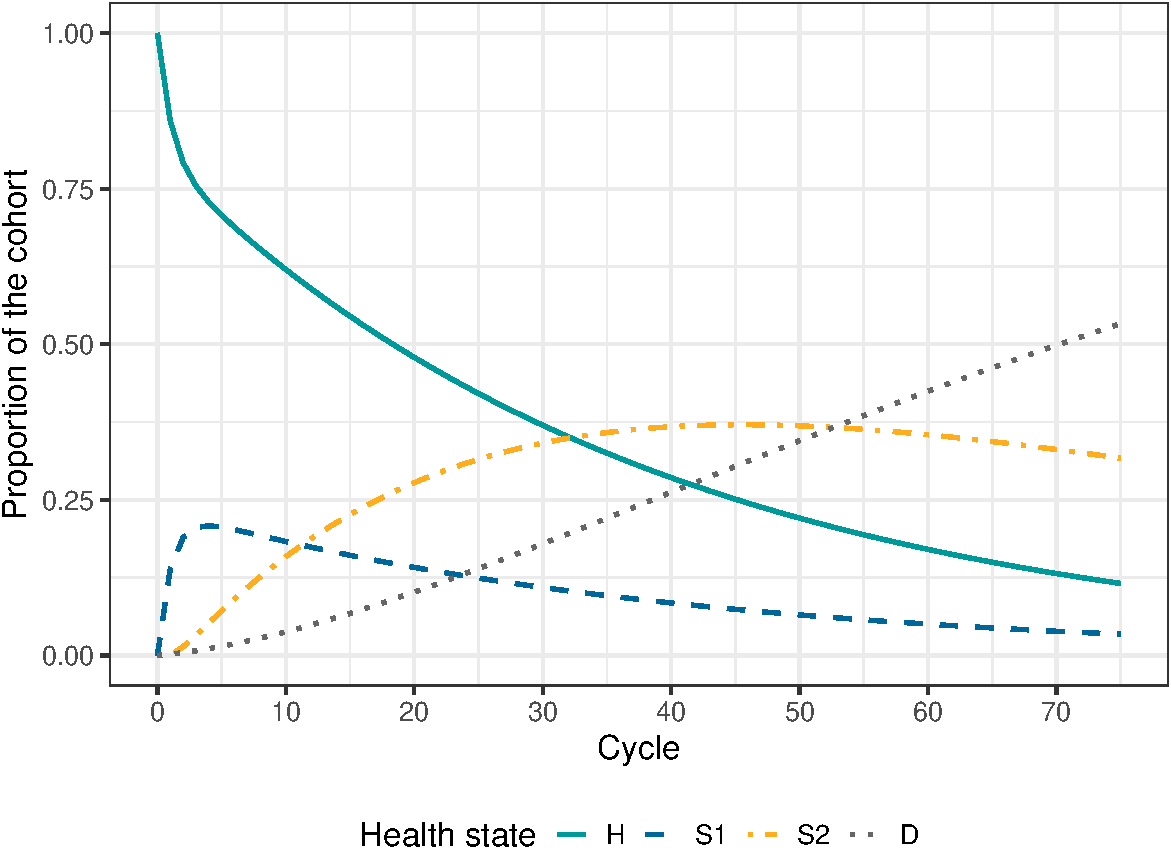
\includegraphics{figs/Sick-Sicker-Trace-TimeHom-1} 

}

\caption{Cohort trace of the time-independent cSTM under strategies SoC and A.}\label{fig:Sick-Sicker-Trace-TimeHom}
\end{figure}

\hypertarget{cost-and-effectiveness-outcomes}{%
\section{Cost and effectiveness outcomes}\label{cost-and-effectiveness-outcomes}}

cSTMs can be used to generate different effectiveness and economic outputs. In a CEA, the outcomes are typically the total expected QALYs and total costs accrued by the cohort over a predefined time horizon. However, epidemiological outcomes are often used to produce other measures of interest or model calibration and validation. Some common epidemiological outcomes include survival, prevalence, incidence, the average number of events, and lifetime risk of events.\textsuperscript{\protect\hyperlink{ref-Siebert2012c}{5}} In this tutorial, we describe how to generate the effectiveness and economic outcomes. In an accompanying tutorial,\textsuperscript{\protect\hyperlink{ref-Alarid-Escudero2021b}{17}} we describe how to compute epidemiological outcomes.

\hypertarget{effectiveness-and-economic-outcomes}{%
\subsection{Effectiveness and economic outcomes}\label{effectiveness-and-economic-outcomes}}

\hypertarget{state-rewards}{%
\subsubsection{State rewards}\label{state-rewards}}

A state reward refers to a value assigned to individuals for being in a given state. In a cost-utility context, these could be either utilities or costs associated with remaining in a certain health state for one cycle. The total expected reward of an outcome of interest for the entire cohort at each cycle can be represented by a column vector \(\mathbf{y}\) of size \(n_T+1\). To calculate \(\mathbf{y}\), we compute the matrix product of the cohort trace matrix times a \emph{vector} of state rewards \(\mathbf{r}\) of the same dimension as the number of states (\(n_S\)), such that
\begin{equation}
  \mathbf{y} = M\mathbf{r}.
  \label{eq:exp-rew-cycle}
\end{equation}
For the Sick-Sicker model, we create a vector of utilities and costs for each of the four strategies considered. The vectors of utilities and costs in R, \texttt{v\_u\_SoC} and \texttt{v\_c\_SoC}, respectively, contain the utilities and costs corresponding with being in each of the four health states under SoC, which are shown in Table \ref{tab:param-table}.

\begin{Shaded}
\begin{Highlighting}[]
\CommentTok{\# Vector of state utilities under SOC}
\NormalTok{v\_u\_SoC }\OtherTok{\textless{}{-}} \FunctionTok{c}\NormalTok{(}\AttributeTok{H =}\NormalTok{ u\_H, }\AttributeTok{S1 =}\NormalTok{ u\_S1, }\AttributeTok{S2 =}\NormalTok{ u\_S2, }\AttributeTok{D =}\NormalTok{ u\_D)}
\CommentTok{\# Vector of state costs under SoC}
\NormalTok{v\_c\_SoC }\OtherTok{\textless{}{-}} \FunctionTok{c}\NormalTok{(}\AttributeTok{H =}\NormalTok{ c\_H, }\AttributeTok{S1 =}\NormalTok{ c\_S1, }\AttributeTok{S2 =}\NormalTok{ c\_S2, }\AttributeTok{D =}\NormalTok{ c\_D)}
\end{Highlighting}
\end{Shaded}

We account for the benefits and costs of both treatments individually and their combination to create the state-reward vectors under treatments A and B (strategies A and B, respectively) and when applied jointly (strategy AB). Only treatment A affects QoL, so we create a vector of utilities for strategy A, \texttt{v\_u\_strA}, where we substitute the utility of being in S1 under SOC, \texttt{u\_S1}, with the utility associated with the benefit of treatment A in being in that state, \texttt{u\_trtA}. Treatment B does not affect QoL, so the vector of utilities for strategy B, \texttt{v\_u\_strB}, is the same as for SoC However, when both treatments A and B are applied jointly (strategy AB), the resulting vector of utilities \texttt{v\_u\_strAB} equals that of strategy A.

\begin{Shaded}
\begin{Highlighting}[]
\CommentTok{\# Vector of state utilities for strategy A}
\NormalTok{v\_u\_strA }\OtherTok{\textless{}{-}} \FunctionTok{c}\NormalTok{(}\AttributeTok{H =}\NormalTok{ u\_H, }\AttributeTok{S1 =}\NormalTok{ u\_trtA, }\AttributeTok{S2 =}\NormalTok{ u\_S2, }\AttributeTok{D =}\NormalTok{ u\_D)}
\CommentTok{\# Vector of state utilities for strategy B}
\NormalTok{v\_u\_strB }\OtherTok{\textless{}{-}}\NormalTok{ v\_u\_SoC}
\CommentTok{\# Vector of state utilities for strategy AB}
\NormalTok{v\_u\_strAB }\OtherTok{\textless{}{-}}\NormalTok{ v\_u\_strA}
\end{Highlighting}
\end{Shaded}

Both treatments A and B incur a cost. To create the vector of state costs for strategy A, \texttt{v\_c\_strA}, we add the cost of treatment A, \texttt{c\_trtA}, to the state costs of S1 and S2. Similarly, when constructing the vector of state costs for strategy B, \texttt{v\_c\_strB}, we add the cost of treatment B, \texttt{c\_trtB}, to the state costs of S1 and S2. Finally, for the vector of state costs for strategy AB, \texttt{v\_c\_strAB}, we add both treatment costs to the state costs of S1 and S2.

\begin{Shaded}
\begin{Highlighting}[]
\CommentTok{\# Vector of state costs for strategy A}
\NormalTok{v\_c\_strA }\OtherTok{\textless{}{-}} \FunctionTok{c}\NormalTok{(}\AttributeTok{H  =}\NormalTok{ c\_H, }
              \AttributeTok{S1 =}\NormalTok{ c\_S1 }\SpecialCharTok{+}\NormalTok{ c\_trtA, }
              \AttributeTok{S2 =}\NormalTok{ c\_S2 }\SpecialCharTok{+}\NormalTok{ c\_trtA, }
              \AttributeTok{D  =}\NormalTok{ c\_D)}
\CommentTok{\# Vector of state costs for strategy B}
\NormalTok{v\_c\_strB }\OtherTok{\textless{}{-}} \FunctionTok{c}\NormalTok{(}\AttributeTok{H  =}\NormalTok{ c\_H, }
              \AttributeTok{S1 =}\NormalTok{ c\_S1 }\SpecialCharTok{+}\NormalTok{ c\_trtB, }
              \AttributeTok{S2 =}\NormalTok{ c\_S2 }\SpecialCharTok{+}\NormalTok{ c\_trtB, }
              \AttributeTok{D  =}\NormalTok{ c\_D)}
\CommentTok{\# Vector of state costs for strategy AB}
\NormalTok{v\_c\_strAB }\OtherTok{\textless{}{-}} \FunctionTok{c}\NormalTok{(}\AttributeTok{H  =}\NormalTok{ c\_H, }
               \AttributeTok{S1 =}\NormalTok{ c\_S1 }\SpecialCharTok{+}\NormalTok{ (c\_trtA }\SpecialCharTok{+}\NormalTok{ c\_trtB), }
               \AttributeTok{S2 =}\NormalTok{ c\_S2 }\SpecialCharTok{+}\NormalTok{ (c\_trtA }\SpecialCharTok{+}\NormalTok{ c\_trtB), }
               \AttributeTok{D  =}\NormalTok{ c\_D)}
\end{Highlighting}
\end{Shaded}

To compute the expected QALYs and costs for the Sick-Sicker model under SoC and strategy A, we apply Equation \eqref{eq:exp-rew-cycle} by multiplying the cohort trace matrix, \texttt{m\_M}, times the corresponding strategy-specific state vectors of rewards. Similarly, To compute the expected rewards for strategies B and AB, we multiply the cohort trace matrix accounting for the effectiveness of treatment B, \texttt{m\_M\_strB}, times their corresponding state vectors of rewards.

\begin{Shaded}
\begin{Highlighting}[]
\CommentTok{\# Vector of QALYs under SoC}
\NormalTok{v\_qaly\_SoC }\OtherTok{\textless{}{-}}\NormalTok{ m\_M }\SpecialCharTok{\%*\%}\NormalTok{ v\_u\_SoC}
\CommentTok{\# Vector of costs under SoC}
\NormalTok{v\_cost\_SoC }\OtherTok{\textless{}{-}}\NormalTok{ m\_M }\SpecialCharTok{\%*\%}\NormalTok{ v\_c\_SoC}
\CommentTok{\# Vector of QALYs for strategy A}
\NormalTok{v\_qaly\_strA }\OtherTok{\textless{}{-}}\NormalTok{ m\_M }\SpecialCharTok{\%*\%}\NormalTok{ v\_u\_strA}
\CommentTok{\# Vector of costs for strategy A}
\NormalTok{v\_cost\_strA }\OtherTok{\textless{}{-}}\NormalTok{ m\_M }\SpecialCharTok{\%*\%}\NormalTok{ v\_c\_strA}
\CommentTok{\# Vector of QALYs for strategy B}
\NormalTok{v\_qaly\_strB }\OtherTok{\textless{}{-}}\NormalTok{ m\_M\_strB }\SpecialCharTok{\%*\%}\NormalTok{ v\_u\_strB}
\CommentTok{\# Vector of costs for strategy B}
\NormalTok{v\_cost\_strB }\OtherTok{\textless{}{-}}\NormalTok{ m\_M\_strB }\SpecialCharTok{\%*\%}\NormalTok{ v\_c\_strB}
\CommentTok{\# Vector of QALYs for strategy AB}
\NormalTok{v\_qaly\_strAB }\OtherTok{\textless{}{-}}\NormalTok{ m\_M\_strB }\SpecialCharTok{\%*\%}\NormalTok{ v\_u\_strAB}
\CommentTok{\# Vector of costs for strategy AB}
\NormalTok{v\_cost\_strAB }\OtherTok{\textless{}{-}}\NormalTok{ m\_M\_strB }\SpecialCharTok{\%*\%}\NormalTok{ v\_c\_strAB}
\end{Highlighting}
\end{Shaded}

\hypertarget{within-cycle-correction}{%
\subsubsection{Within-cycle correction}\label{within-cycle-correction}}

Discretizing a continuous-time cSTM with a discrete-time cSTM might introduce biases in the time spent on each state.\textsuperscript{\protect\hyperlink{ref-VanRosmalen2013}{21}} One approach to reducing these biases is to reduce cycle length, which will require simulating the model for a larger number of cycles, which sometimes is not computationally efficient. Another approach to better approximate the expected rewards of cumulative health and cost outcomes from a continuous-time process using a discrete-time model is to use within-cycle corrections (WCC).\textsuperscript{\protect\hyperlink{ref-Hunink2014}{22}} In this tutorial, we use Simpson's 1/3rd rule as a WCC by multiplying the rewards (e.g., costs and effectiveness) by \(1/3\) in the first and last cycles, by \(4/3\) if cycle number is odd, and by \(2/3\) if the cycle number is even.\textsuperscript{\protect\hyperlink{ref-Elbasha2016a}{24}} We implement the WCC by generating a column vector \(\mathbf{wcc}\) of size \(n_T+1\) with values corresponding to the first, \(t=0\), and last cycle, \(t= n_T + 1\), equal to \(1/3\), and the entries corresponding to the even and odd cycles with \(2/3\) and \(4/3\), respectively.

\[
  \mathbf{wcc} = \left[\frac{1}{3}, \frac{2}{3}, \frac{4}{3}, \cdots, \frac{1}{3}\right]
\]

The within-cycle correction vector is the same for both costs and QALYs; thus, only one vector, \texttt{v\_wcc}, is required.

\begin{Shaded}
\begin{Highlighting}[]
\DocumentationTok{\#\# Vector with cycles}
\NormalTok{v\_cycles }\OtherTok{\textless{}{-}} \FunctionTok{seq}\NormalTok{(}\DecValTok{1}\NormalTok{, n\_cycles }\SpecialCharTok{+} \DecValTok{1}\NormalTok{)}
\DocumentationTok{\#\# Generate 2/3 and 4/3 multipliers for even and odd entries, respectively}
\NormalTok{v\_wcc }\OtherTok{\textless{}{-}}\NormalTok{ ((v\_cycles }\SpecialCharTok{\%\%} \DecValTok{2}\NormalTok{) }\SpecialCharTok{==} \DecValTok{0}\NormalTok{)}\SpecialCharTok{*}\NormalTok{(}\DecValTok{2}\SpecialCharTok{/}\DecValTok{3}\NormalTok{) }\SpecialCharTok{+}\NormalTok{ ((v\_cycles }\SpecialCharTok{\%\%} \DecValTok{2}\NormalTok{) }\SpecialCharTok{!=} \DecValTok{0}\NormalTok{)}\SpecialCharTok{*}\NormalTok{(}\DecValTok{4}\SpecialCharTok{/}\DecValTok{3}\NormalTok{)}
\DocumentationTok{\#\# Substitute 1/3 in first and last entries}
\NormalTok{v\_wcc[}\DecValTok{1}\NormalTok{] }\OtherTok{\textless{}{-}}\NormalTok{ v\_wcc[n\_cycles }\SpecialCharTok{+} \DecValTok{1}\NormalTok{] }\OtherTok{\textless{}{-}} \DecValTok{1}\SpecialCharTok{/}\DecValTok{3}
\end{Highlighting}
\end{Shaded}

\hypertarget{discounting-future-rewards}{%
\subsubsection{Discounting future rewards}\label{discounting-future-rewards}}

Future costs and benefits are often discounted by a specific rate to calculate the net present value of these rewards. To account for discounting, the generated rewards per cycle are multiplied by the cycle-specific discount weight. The vector of expected rewards, \(\mathbf{y}\), is multiplied by a discounting column vector \(\mathbf{d}\) of size \(n_T+1\) where each of its \(t\)-th entry represents the discounting for cycle \(t\)
\[
  \mathbf{d} = \left[1, \frac{1}{(1+d)^{1}}, \frac{1}{(1+d)^{2}}, \cdots, \frac{1}{(1+d)^{n_T}}\right],
\]
where \(d\) is the cycle-length discount rate. Therefore, the total expected discounted outcome over the \(n_T\) cycles, \(y\), is obtained by the inner product between \(\mathbf{y}\) transposed, \(\mathbf{y'}\), and \(\mathbf{d}\),
\begin{equation}
 y = \mathbf{y'} \mathbf{d}.
 \label{eq:tot-exp-disc-rewd}
\end{equation}
The discount vectors for costs and QALYs for the Sick-Sicker model, \texttt{v\_dwc} and \texttt{v\_dwe}, respectively, are

\begin{Shaded}
\begin{Highlighting}[]
\CommentTok{\# Discount weight for effects}
\NormalTok{v\_dwe }\OtherTok{\textless{}{-}} \DecValTok{1} \SpecialCharTok{/}\NormalTok{ ((}\DecValTok{1} \SpecialCharTok{+}\NormalTok{ d\_e) }\SpecialCharTok{\^{}}\NormalTok{ (}\DecValTok{0}\SpecialCharTok{:}\NormalTok{(n\_cycles)))  }
\CommentTok{\# Discount weight for costs }
\NormalTok{v\_dwc }\OtherTok{\textless{}{-}} \DecValTok{1} \SpecialCharTok{/}\NormalTok{ ((}\DecValTok{1} \SpecialCharTok{+}\NormalTok{ d\_c) }\SpecialCharTok{\^{}}\NormalTok{ (}\DecValTok{0}\SpecialCharTok{:}\NormalTok{(n\_cycles)))    }
\end{Highlighting}
\end{Shaded}

To account for both discounting and within-cycle correction, we incorporate \(\mathbf{wcc}\) in equation \eqref{eq:tot-exp-disc-rewd} using an element-wise multiplication with \(\mathbf{d}\), indicated by the \(\odot\) sign.
\begin{equation}
 y = \mathbf{y}^{'} \left(\mathbf{d} \odot \mathbf{wcc}\right).
 \label{eq:tot-exp-disc-rewd-wcc}
\end{equation}

To compute the total expected discounted QALYs and costs under all four strategies accounting for within-cycle correction, we apply Equation \eqref{eq:tot-exp-disc-rewd-wcc} to the vectors with the rewards, discounts, and within-cycle correction.

\begin{Shaded}
\begin{Highlighting}[]
\DocumentationTok{\#\# Expected discounted QALYs under SoC}
\NormalTok{n\_tot\_qaly\_SoC }\OtherTok{\textless{}{-}} \FunctionTok{t}\NormalTok{(v\_qaly\_SoC) }\SpecialCharTok{\%*\%}\NormalTok{ (v\_dwe }\SpecialCharTok{*}\NormalTok{ v\_wcc)}
\DocumentationTok{\#\# Expected discounted costs under SoC}
\NormalTok{n\_tot\_cost\_SoC }\OtherTok{\textless{}{-}} \FunctionTok{t}\NormalTok{(v\_cost\_SoC) }\SpecialCharTok{\%*\%}\NormalTok{ (v\_dwc }\SpecialCharTok{*}\NormalTok{ v\_wcc)}
\DocumentationTok{\#\# Expected discounted QALYs for strategy A}
\NormalTok{n\_tot\_qaly\_strA }\OtherTok{\textless{}{-}} \FunctionTok{t}\NormalTok{(v\_qaly\_strA) }\SpecialCharTok{\%*\%}\NormalTok{ (v\_dwe }\SpecialCharTok{*}\NormalTok{ v\_wcc)}
\DocumentationTok{\#\# Expected discounted costs for strategy A}
\NormalTok{n\_tot\_cost\_strA }\OtherTok{\textless{}{-}} \FunctionTok{t}\NormalTok{(v\_cost\_strA) }\SpecialCharTok{\%*\%}\NormalTok{ (v\_dwc }\SpecialCharTok{*}\NormalTok{ v\_wcc)}
\DocumentationTok{\#\# Expected discounted QALYs for strategy B}
\NormalTok{n\_tot\_qaly\_strB }\OtherTok{\textless{}{-}} \FunctionTok{t}\NormalTok{(v\_qaly\_strB) }\SpecialCharTok{\%*\%}\NormalTok{ (v\_dwe }\SpecialCharTok{*}\NormalTok{ v\_wcc)}
\DocumentationTok{\#\# Expected discounted costs for strategy B}
\NormalTok{n\_tot\_cost\_strB }\OtherTok{\textless{}{-}} \FunctionTok{t}\NormalTok{(v\_cost\_strB) }\SpecialCharTok{\%*\%}\NormalTok{ (v\_dwc }\SpecialCharTok{*}\NormalTok{ v\_wcc)}
\DocumentationTok{\#\# Expected discounted QALYs for strategy AB}
\NormalTok{n\_tot\_qaly\_strAB }\OtherTok{\textless{}{-}} \FunctionTok{t}\NormalTok{(v\_qaly\_strAB) }\SpecialCharTok{\%*\%}\NormalTok{ (v\_dwe }\SpecialCharTok{*}\NormalTok{ v\_wcc)}
\DocumentationTok{\#\# Expected discounted costs for strategy AB}
\NormalTok{n\_tot\_cost\_strAB }\OtherTok{\textless{}{-}} \FunctionTok{t}\NormalTok{(v\_cost\_strAB) }\SpecialCharTok{\%*\%}\NormalTok{ (v\_dwc }\SpecialCharTok{*}\NormalTok{ v\_wcc)}
\end{Highlighting}
\end{Shaded}

\begin{table}[!h]

\caption{\label{tab:Expected-outcomes-table}Total expected discounted QALYs and costs per average individual in the cohort of the Sick-Sicker model by strategy accounting for within-cycle correction.}
\centering
\begin{tabular}[t]{llc}
\toprule
  & Costs & QALYs\\
\midrule
Standard of care & \$148,657 & 20.990\\
Strategy A & \$275,937 & 21.717\\
Strategy B & \$248,571 & 22.482\\
Strategy AB & \$361,341 & 23.354\\
\bottomrule
\end{tabular}
\end{table}

The total expected discounted QALYs and costs for the Sick-Sicker model under the four strategies accounting for within-cycle correction are shown in Table \ref{tab:Expected-outcomes-table}.

\hypertarget{cost-effectiveness-analysis-and-incremental-cost-effectiveness-ratios-icers}{%
\section{Cost-effectiveness analysis and incremental cost-effectiveness ratios (ICERs)}\label{cost-effectiveness-analysis-and-incremental-cost-effectiveness-ratios-icers}}

We combine the total expected discounted costs and QALYs for all four strategies into outcome-specific vectors, \texttt{v\_cost\_str} for costs and \texttt{v\_qaly\_str} for QALYs. We use the R package \texttt{dampack} (\url{https://cran.r-project.org/web/packages/dampack/})\textsuperscript{\protect\hyperlink{ref-Alarid-Escudero2021}{25}} to calculate the incremental costs and effectiveness and the incremental cost-effectiveness ratio (ICER) the non-dominated strategies and create the data frame \texttt{df\_cea} with this information.

\begin{Shaded}
\begin{Highlighting}[]
\DocumentationTok{\#\#\# Vector of costs}
\NormalTok{v\_cost\_str }\OtherTok{\textless{}{-}} \FunctionTok{c}\NormalTok{(n\_tot\_cost\_SoC, n\_tot\_cost\_strA, n\_tot\_cost\_strB, n\_tot\_cost\_strAB)}
\DocumentationTok{\#\#\# Vector of effectiveness}
\NormalTok{v\_qaly\_str }\OtherTok{\textless{}{-}} \FunctionTok{c}\NormalTok{(n\_tot\_qaly\_SoC, n\_tot\_qaly\_strA, n\_tot\_qaly\_strB, n\_tot\_qaly\_strAB)}

\DocumentationTok{\#\#\# Calculate incremental cost{-}effectiveness ratios (ICERs)}
\NormalTok{df\_cea }\OtherTok{\textless{}{-}}\NormalTok{ dampack}\SpecialCharTok{::}\FunctionTok{calculate\_icers}\NormalTok{(}\AttributeTok{cost =}\NormalTok{ v\_cost\_str, }
                                   \AttributeTok{effect =}\NormalTok{ v\_qaly\_str,}
                                   \AttributeTok{strategies =}\NormalTok{ v\_names\_str)}
\end{Highlighting}
\end{Shaded}

The CEA results of the Sick-Sicker model are presented in Table \ref{tab:table-cea}. SoC is the least costly and effective strategy, followed by Strategy B producing an expected incremental benefit of 1.492 QALYs per individual for an additional expected cost of \$99,913 with an ICER of \$66,960/QALY followed by Strategy AB with an ICER \$129,354/QALY. Strategy A is a dominated strategy.

\begin{table}[!h]

\caption{\label{tab:table-cea}Cost-effectiveness analysis results for the Sick-Sicker model. ND: Non-dominated strategy; D: Dominated strategy.}
\centering
\begin{tabular}[t]{rcccccc}
\toprule
Strategy & Costs (\$) & QALYs & Incremental Costs (\$) & Incremental QALYs & ICER (\$/QALY) & Status\\
\midrule
Standard of care & 148,657 & 20.990 & NA & NA & NA & ND\\
Strategy B & 248,571 & 22.482 & 99,913 & 1.492 & 66,960 & ND\\
Strategy AB & 361,341 & 23.354 & 112,771 & 0.872 & 129,354 & ND\\
Strategy A & 275,937 & 21.717 & NA & NA & NA & D\\
\bottomrule
\end{tabular}
\end{table}

Figure \ref{fig:Sick-Sicker-CEA} shows the cost-effectiveness efficient frontier of all four strategies for the time-independent Sick-Sicker model.

\begin{figure}[H]

{\centering 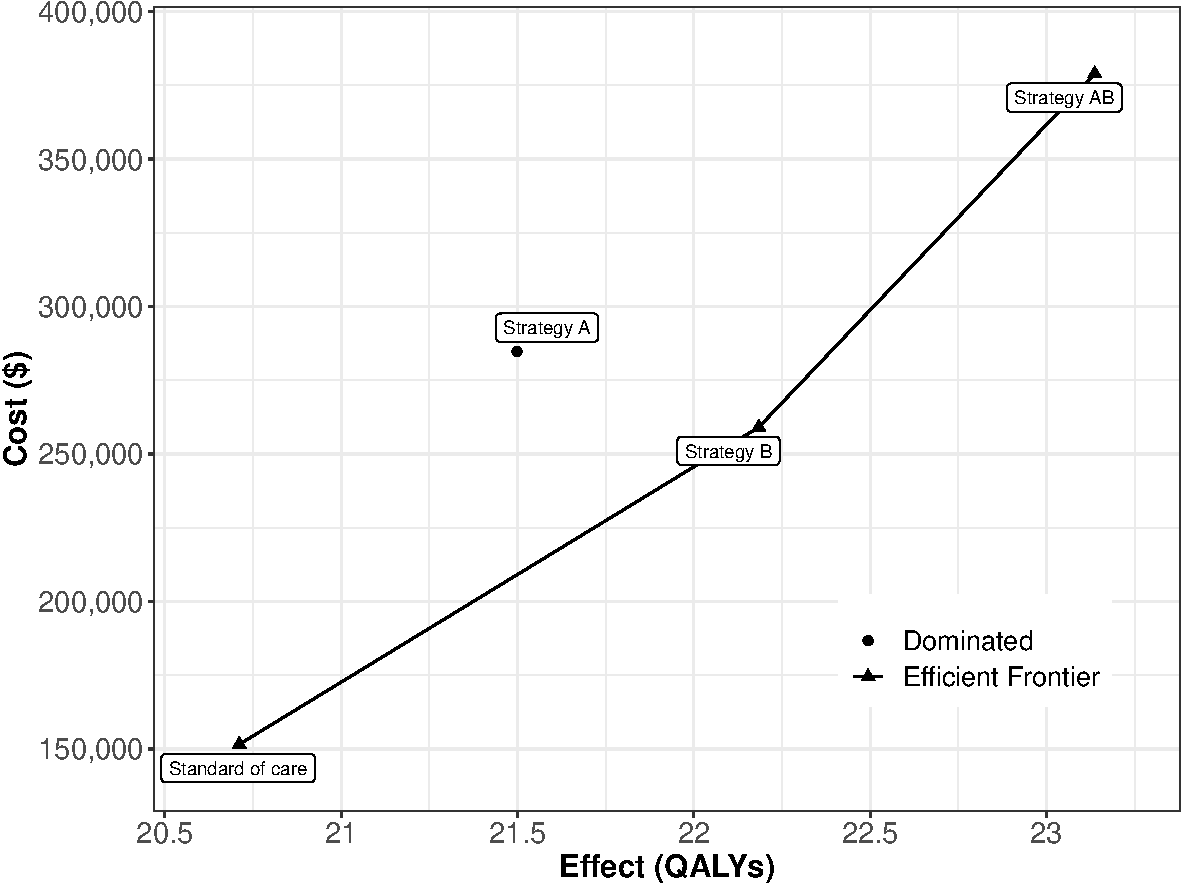
\includegraphics{figs/Sick-Sicker-CEA-1} 

}

\caption{Cost-effectiveness efficient frontier of all four strategies for the time-independent Sick-Sicker model.}\label{fig:Sick-Sicker-CEA}
\end{figure}

\hypertarget{probabilistic-sensitivity-analysis}{%
\section{Probabilistic sensitivity analysis}\label{probabilistic-sensitivity-analysis}}

To quantify the effect of model parameter uncertainty on cost-effectiveness outcomes, we conducted a probabilistic sensitivity analysis (PSA).\textsuperscript{\protect\hyperlink{ref-Briggs2012}{26}} In a PSA, we randomly draw parameter sets from distributions that reflect the current uncertainty in model parameter estimates. The distribution for all the parameters and their values are described in Table \ref{tab:param-table} and more detailed in the Supplementary Material. For each sampled set of parameter values, we compute model outcomes (e.g., total discounted cost and QALYs) for each strategy. In a previously published manuscript, we describe the implementation of these steps in R.\textsuperscript{\protect\hyperlink{ref-Alarid-Escudero2019e}{20}} Briefly, to conduct the PSA, we create three R functions:

\begin{enumerate}
\def\labelenumi{\arabic{enumi}.}
\tightlist
\item
  A function called \texttt{generate\_psa\_params(n\_sim,\ seed)} with arguments \texttt{n\_sim} and \texttt{seed}. The function generates a sample of size \texttt{n\_sim} for the model parameters from their distributions defined in Table \ref{tab:param-table}. The function also takes a seed number as input, \texttt{seed}, which ensures reproducibility of the PSA results. By calling this function, we generate the sample of parameter sets for the PSA, \texttt{df\_psa\_input}, via: \texttt{df\_psa\_input\ \textless{}-\ generate\_psa\_params(n\_sim\ =\ n\_sim)}.
\item
  A function called \texttt{decision\_model(l\_params\_all)} that wraps the R code of the time-independent cSTM described in section \protect\hyperlink{conceptualizing-and-implementing-time-independent-cSTM-dynamics}{Conceptualizing and implementing time-independent cSTM dynamics}. This function requires inputting a list of all model parameter values, \texttt{l\_params\_all} and whether the user wants print messages via the \texttt{verbose} parameter.
\item
  A function called \texttt{calculate\_ce\_out(l\_params\_all,\ n\_wtp\ =\ 100000)} that calculates total discounted costs and QALYs based on the \texttt{decision\_model} function output. This function also computes the net monetary benefit (NMB) for a given willingness-to-pay threshold, specified by the argument \texttt{n\_wtp}.
  These functions are provided in the Supplementary Material and the accompanying GitHub repository of this manuscript.
\end{enumerate}

To conduct the PSA of the CEA using the time-independent Sick-Sicker cSTM, we sampled 1,000 parameter sets for all the parameters from the distributions defined in Table \ref{tab:param-table}. For each sampled parameter set, we simulated each strategy. Results from a PSA can be represented in various ways. For example, the joint distribution, 95\% confidence ellipse, and the expected values of the total discounted costs and QALYs for each strategy can be plotted in a cost-effectiveness (CE) scatter plot ( Figure \ref{fig:CE-scatter}),\textsuperscript{\protect\hyperlink{ref-Briggs2002}{27}} where each of the 1,000 simulations are plotted as a point in the graph. The CE scatter plot for CEA using the time-independent model shows that strategy AB has the highest expected costs and QALYs. Standard of care has the lowest expected cost and QALYs. Strategy B is more effective and least costly than Strategy A. Strategy A is a strongly dominated strategy.

\begin{figure}[H]

{\centering 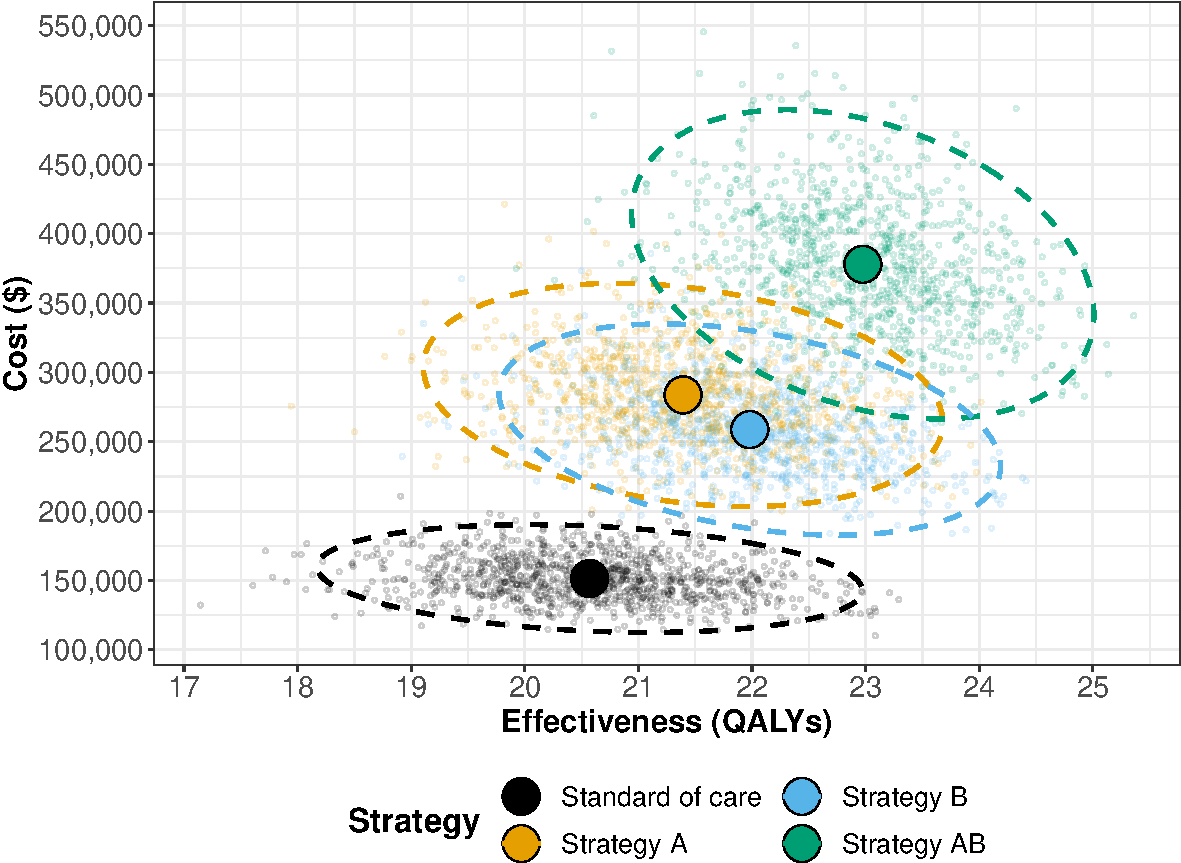
\includegraphics{figs/CE-scatter-1} 

}

\caption{Cost-effectiveness scatter plot.}\label{fig:CE-scatter}
\end{figure}

In Figure \ref{fig:CEAC}, we present the cost-effectiveness acceptability curves (CEACs), which shows the probability that each strategy is cost-effective, and the cost-effectiveness frontier (CEAF), which shows the strategy with the highest expected monetary benefit, over a range of willingness-to-pay (WTP) thresholds. Each strategy's net monetary benefit (NMB) is defined as the product of total discounted QALYs and the WTP threshold minus the total discounted costs,\textsuperscript{\protect\hyperlink{ref-Stinnett1998b}{28}} calculated for each PSA parameter set sample. At WTP thresholds less than \$70,000 per QALY, SoC is the strategy with the highest probability of being cost-effective and the highest expected NMB. Strategy B has the highest probability of being cost-effective and the highest expected NMB for WTP thresholds between \$70,000 and \$125,000 per QALY. Strategy AB has the highest expected NMB for WTP thresholds greater than or equal to \$125,000 per QALY and is the strategy with the highest probability of being cost-effective.

\begin{figure}[H]

{\centering 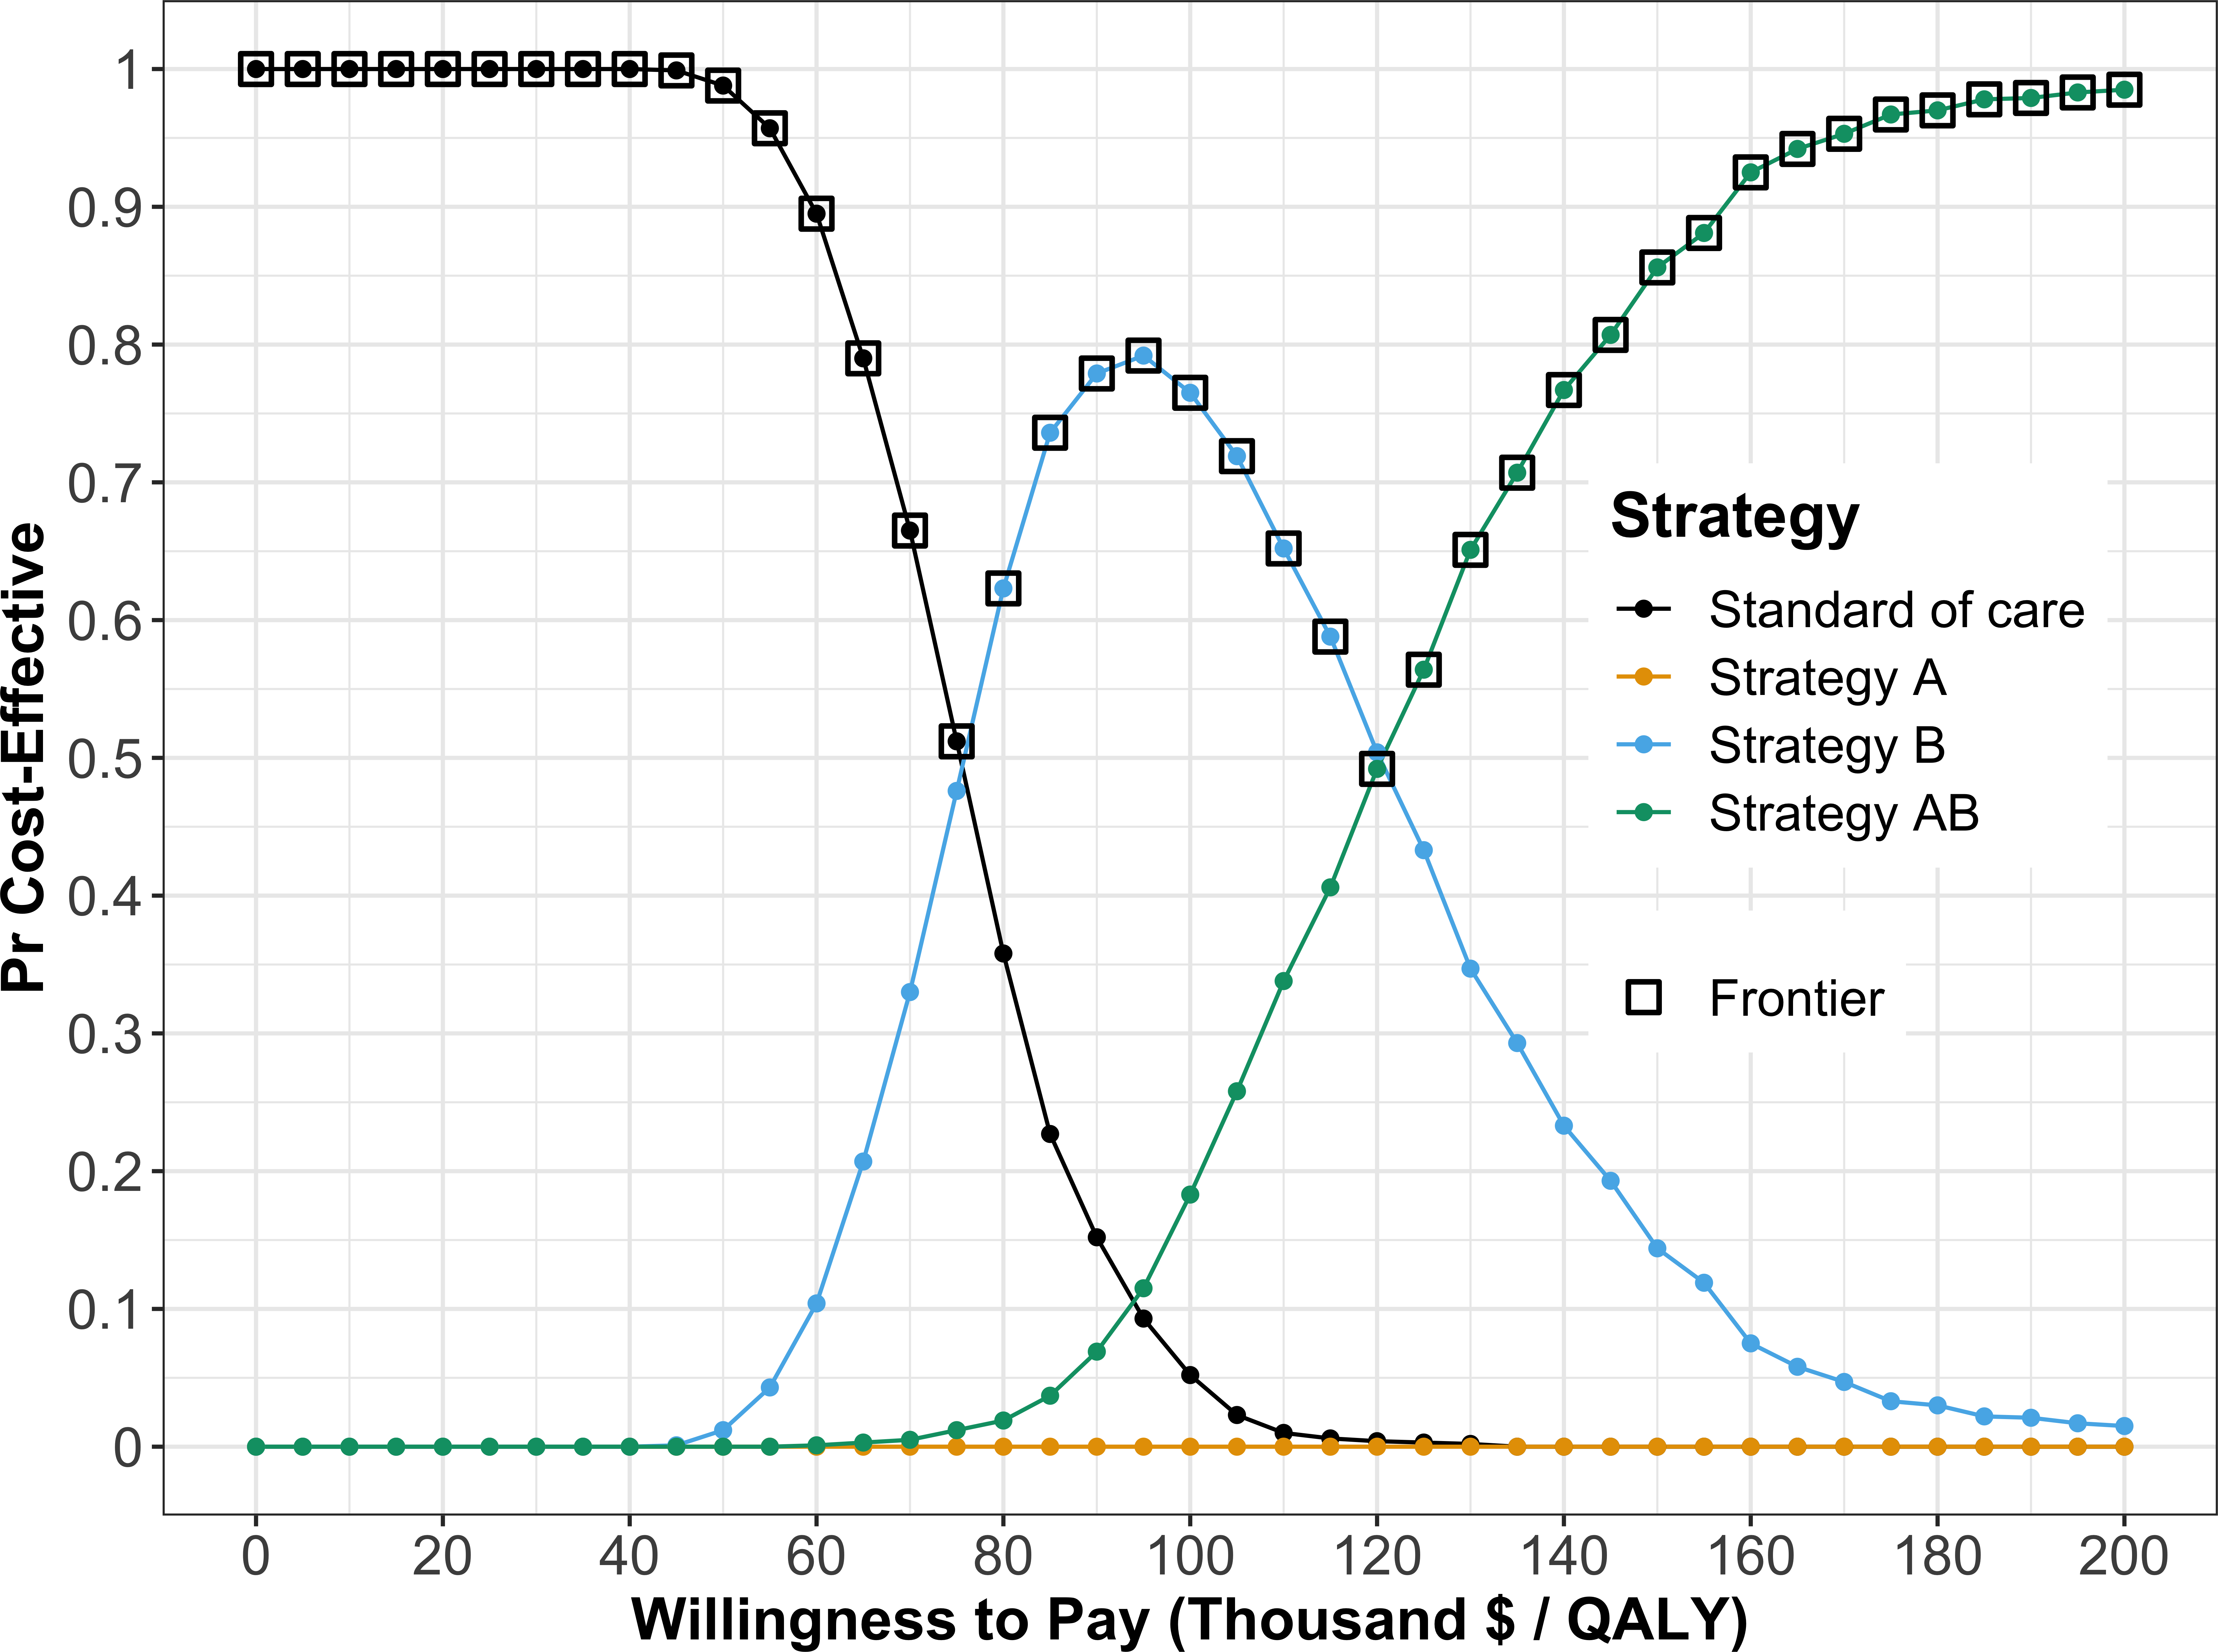
\includegraphics{figs/CEAC-1} 

}

\caption{Cost-effectiveness acceptability curves (CEACs) and frontier (CEAF).}\label{fig:CEAC}
\end{figure}

The code provided in the GitHub repository also produces expected loss curves (ELCs). These curves quantify the expected loss from each strategy over a range of WTP thresholds (Figure \ref{fig:ELC}). The expected loss considers both the probability of making the wrong decision and the magnitude of the loss due to this decision, representing the foregone benefits of choosing a suboptimal strategy. The expected loss of the optimal strategy represents the lowest envelope of the ELCs because, given current information, the loss cannot be minimized further. The lower envelope also represents the expected value of perfect information (EVPI), which quantifies the value of eliminating parameter uncertainty. The strategy SoC has the lowest expected loss for WTP thresholds less than \$65,000 per QALY, strategy B has the lowest expected loss for WTP threshold greater than or equal to \$70,000 and less than \$125,000. Strategy AB has the lowest expected loss for WTP threshold greater than or equal to \$125,000 per QALY. At a WTP threshold of \$125,000 per QALY, the EVPI is highest at \$9,577. For a more detailed description of these outputs and the R code to generate them, we refer the reader to a previous publication by our group.\textsuperscript{\protect\hyperlink{ref-Alarid-Escudero2019}{29}}

\begin{figure}[H]

{\centering 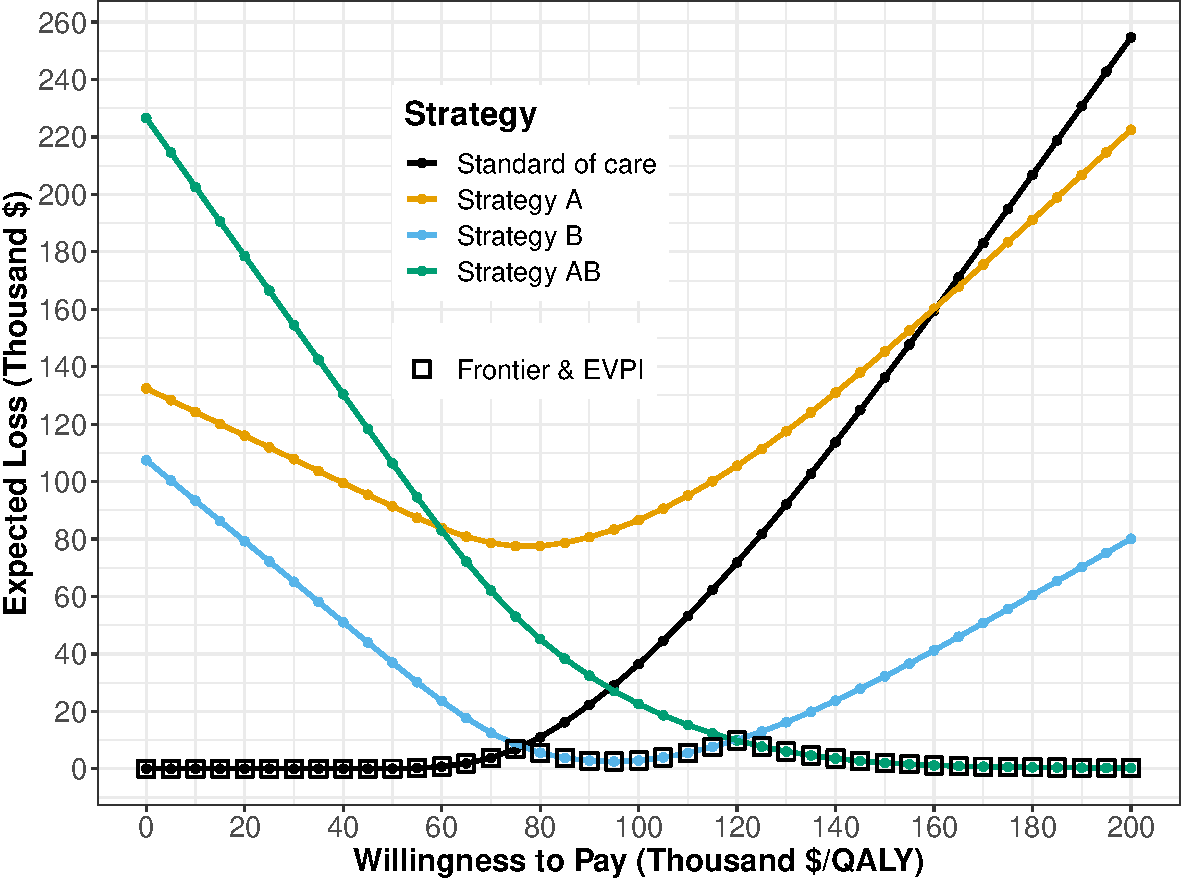
\includegraphics{figs/ELC-1} 

}

\caption{Expected loss curves (ELCs) and expected value of perfect information (EVPI).}\label{fig:ELC}
\end{figure}

\hypertarget{discussion}{%
\section{Discussion}\label{discussion}}

In this tutorial, we provided a conceptualization of time-independent cSTMs with their mathematical description and a walk-through of their implementation for CEA in R using a previously published example. We used R as the programming language of choice to show these models' implementation with accompanying code throughout the tutorial.

The parameterization of our example model assumes all parameters are known, or at least, the characterization of their uncertainty is known (i.e., we know their distributions). However, to construct a real-world cSTM, modelers must conduct a thorough synthesis of current evidence to determine these models' appropriate structure and inform all parameters. For example, determining whether transitions between non-death health states are estimated conditional on being alive or mortality risks are also considered competing risks.\textsuperscript{\protect\hyperlink{ref-Briggs2012}{26}} Similarly, our PSA analysis simplifies reality where all model parameters are assumed to be independent of each other. However, parameters could be correlated with each other or have a rank order, and appropriate statistical methods that simulate these correlations or rank order might be needed.\textsuperscript{\protect\hyperlink{ref-Goldhaber-Fiebert2015}{30}} We encourage modelers to use appropriate statistical methods to synthesize and quantify model parameters uncertainty accurately. Besides, modelers should correctly specify all model parameters for the cycle length of the model. For example, some probability revision is required to adjust an annual mortality rate to a weekly probability correctly.\textsuperscript{\protect\hyperlink{ref-Hunink2014}{22}}

In general, cSTMs are recommended when the number of states is ``not too large''.\textsuperscript{\protect\hyperlink{ref-Siebert2012c}{5}} This recommendation arises because as the number of states increases, it becomes more difficult to keep track of their construction but not because of the added computational expense. It is possible to build fairly complex cSTMs in R as long as the size of the transition probability matrix and outputs of interest can be stored in the RAM memory of the computer running the analysis. For example, a typical PC with 8GB of RAM can handle a transition probability array of about 1000 states and 600 slices. However, these matrices can grow quickly, and if the required number of state descriptions gets too large and difficult to manage its coding, it becomes preferable to use a stochastic (Monte Carlo) version of the state-transition model --often called individual-based state-transition models (iSTM) or microsimulation models-- rather than a cohort simulation model.\textsuperscript{\protect\hyperlink{ref-Siebert2012c}{5}} In iSTM, the risks and rewards of simulated individuals do not need to depend only on a specific health state and can depend on their individual characteristics and attributes. Besides, modelers can store health state history and other events over time for each individual to determine the risk of new events and corresponding costs and effects. It is recommended to think about the required model structure before implementing the model in R or any other tool because turning a cSTM into an iSTM requires a different code structure. However, most input parameters and some model structures might remain the same. Still, an iSTM will also require additional functions to describe the dependency of transition probabilities and rewards on individuals' history. In a previous tutorial, we showed how to write these additional functions for the Sick-Sicker example model.\textsuperscript{\protect\hyperlink{ref-Krijkamp2018}{6}}

With increasing model complexity and interdependency of functions to conduct various analyses like PSA, it is important to ensure all code and functions work as expected and all elements of cSTM are valid. We can achieve this by creating functions that help with model debugging and validation and thorough unit testing. In the accompanying GitHub repository, we provided functions to check that transition probability matrices and their elements are valid. However, unit testing is beyond the scope of this tutorial. Still, we refer the reader to a previously published manuscript where we describe unit testing in more detail and provide accompanying code.\textsuperscript{\protect\hyperlink{ref-Alarid-Escudero2019e}{20}}

We focused on discrete-time matrix-form cSTMs, but these can also be implemented via a set of difference equations and continuous-time using differential equations in R.\textsuperscript{\protect\hyperlink{ref-Grimmett2014}{31},\protect\hyperlink{ref-Axler2005}{32}} We refer readers interested in learning more on continuous-time cSTMs to previously published manuscripts\textsuperscript{\protect\hyperlink{ref-VanRosmalen2013}{21},\protect\hyperlink{ref-Cao2016}{33}--\protect\hyperlink{ref-Soares2012}{35}} and a tutorial using R.\textsuperscript{\protect\hyperlink{ref-Frederix2013a}{36}} This tutorial shows how cSTMs are constructed, parameterized, and run using only base R, so readers get a deep understanding of this type of decision model. Finally, the variable names used in this paper reflect our style. While we provide standardized variable names, adopting these conventions is ultimately a personal preference.

In summary, this tutorial provides a conceptualization of time-independent cSTMs and a step-by-step guide to implement them in R. We aim to add to the current body of literature and material on building this type of decision model, so health decision scientists and health economists can develop cSTMs in a more flexible, efficient, open-source manner and encourage increased transparency and reproducibility.

\hypertarget{acknowledgements}{%
\section{Acknowledgements}\label{acknowledgements}}

Dr.~Alarid-Escudero was supported by a grant from the National Cancer Institute (U01-CA-199335) as part of the Cancer Intervention and Surveillance Modeling Network (CISNET) and the Gordon and Betty Moore Foundation. Miss Krijkamp was supported by a fellowship from a grant by the Gordon and Betty Moore Foundation (GBMF7853) through the Society for Medical Decision Making (SMDM). Dr.~Enns was supported by a grant from the National Institute of Allergy and Infectious Diseases of the National Institutes of Health under award no. K25AI118476. Dr.~Hunink receives Royalties from Cambridge University Press for a textbook on Medical Decision Making, reimbursement of expenses from the European Society of Radiology (ESR) for work on the ESR guidelines for imaging referrals, reimbursement of expenses from the European Institute for Biomedical Imaging Research (EIBIR) for membership of the Scientific Advisory Board, and research funding from the American Diabetes Association, the Netherlands Organization for Health Research and Development, the German Innovation Fund, Netherlands Educational Grant (``Studie Voorschot Middelen''), and the Gordon and Betty Moore Foundation. Dr.~Jalal was supported by a grant from the National Institute on Drug Abuse of the National Institute of Health under award no. K01DA048985. The content is solely the authors' responsibility and does not necessarily represent the official views of the National Institutes of Health. The funding agencies had no role in the study's design, interpretation of results, or writing of the manuscript. The funding agreement ensured the authors' independence in designing the study, interpreting the data, writing, and publishing the report. We also want to thank the anonymous reviewers of \emph{Medical Decision Making} for their valuable suggestions and the students who have taken our classes and provided invaluable feedback to improve the clarity and usability of our materials.

\hypertarget{references}{%
\section*{References}\label{references}}
\addcontentsline{toc}{section}{References}

\hypertarget{refs}{}
\begin{CSLReferences}{0}{0}
\leavevmode\hypertarget{ref-Kuntz2017}{}%
\CSLLeftMargin{1. }
\CSLRightInline{Kuntz KM, Russell LB, Owens DK, et al. {Decision Models in Cost-Effectiveness Analysis}. In: Neumann PJ, Sanders GD, Russell LB, et al. (eds) \emph{Cost-effectiveness in health and medicine}. New York, NY: Oxford University Press, 2017, pp. 105--136.}

\leavevmode\hypertarget{ref-Jalal2017b}{}%
\CSLLeftMargin{2. }
\CSLRightInline{Jalal H, Pechlivanoglou P, Krijkamp E, et al. {An Overview of R in Health Decision Sciences}. \emph{Medical Decision Making}; 37: 735--746, \url{http://journals.sagepub.com/doi/10.1177/0272989X16686559} (2017).}

\leavevmode\hypertarget{ref-Spedicato2017}{}%
\CSLLeftMargin{3. }
\CSLRightInline{Spedicato GA. {Discrete Time Markov Chains with R}. \emph{The R Journal}; 9: 84--104, \url{https://journal.r-project.org/archive/2017/RJ-2017-036/RJ-2017-036.pdf} (2017).}

\leavevmode\hypertarget{ref-Filipovic-Pierucci2017}{}%
\CSLLeftMargin{4. }
\CSLRightInline{Filipović-Pierucci A, Zarca K, Durand-Zaleski I. {Markov Models for Health Economic Evaluation: The R Package heemod}. \emph{arXiv:170203252v1}; April: 30, \url{http://arxiv.org/abs/1702.03252} (2017).}

\leavevmode\hypertarget{ref-Siebert2012c}{}%
\CSLLeftMargin{5. }
\CSLRightInline{Siebert U, Alagoz O, Bayoumi AM, et al. {State-Transition Modeling: A Report of the ISPOR-SMDM Modeling Good Research Practices Task Force-3}. \emph{Medical Decision Making}; 32: 690--700, \url{http://mdm.sagepub.com/cgi/doi/10.1177/0272989X12455463} (2012).}

\leavevmode\hypertarget{ref-Krijkamp2018}{}%
\CSLLeftMargin{6. }
\CSLRightInline{Krijkamp EM, Alarid-Escudero F, Enns EA, et al. {Microsimulation Modeling for Health Decision Sciences Using R: A Tutorial}. \emph{Medical Decision Making}; 38: 400--422, \url{http://journals.sagepub.com/doi/10.1177/0272989X18754513} (2018).}

\leavevmode\hypertarget{ref-Suijkerbuijk2018}{}%
\CSLLeftMargin{7. }
\CSLRightInline{Suijkerbuijk AWM, Van Hoek AJ, Koopsen J, et al. {Cost-effectiveness of screening for chronic hepatitis B and C among migrant populations in a low endemic country}. \emph{PLoS ONE} 2018; 13: 1--16.}

\leavevmode\hypertarget{ref-Sathianathen2018a}{}%
\CSLLeftMargin{8. }
\CSLRightInline{Sathianathen NJ, Konety BR, Alarid-Escudero F, et al. {Cost-effectiveness Analysis of Active Surveillance Strategies for Men with Low-risk Prostate Cancer}. \emph{European Urology}; 75: 910--917, \url{https://linkinghub.elsevier.com/retrieve/pii/S0302283818308534} (2019).}

\leavevmode\hypertarget{ref-Lu2018b}{}%
\CSLLeftMargin{9. }
\CSLRightInline{Lu S, Yu Y, Fu S, et al. {Cost-effectiveness of ALK testing and first-line crizotinib therapy for non-small-cell lung cancer in China}. \emph{PLoS ONE} 2018; 13: 1--12.}

\leavevmode\hypertarget{ref-Djatche2018}{}%
\CSLLeftMargin{10. }
\CSLRightInline{Djatche LM, Varga S, Lieberthal RD. {Cost-Effectiveness of Aspirin Adherence for Secondary Prevention of Cardiovascular Events}. \emph{PharmacoEconomics - Open}; 2: 371--380, \url{https://doi.org/10.1007/s41669-018-0075-2} (2018).}

\leavevmode\hypertarget{ref-Smith-Spangler2010}{}%
\CSLLeftMargin{11. }
\CSLRightInline{Smith-Spangler CM, Juusola JL, Enns EA, et al. {Population Strategies to Decrease Sodium Intake and the Burden of Cardiovascular Disease: A Cost-Effectiveness Analysis}. \emph{Annals of Internal Medicine}; 152: 481--487, \url{http://annals.org/article.aspx?articleid=745729} (2010).}

\leavevmode\hypertarget{ref-Pershing2014}{}%
\CSLLeftMargin{12. }
\CSLRightInline{Pershing S, Enns EA, Matesic B, et al. {Cost-Effectiveness of Treatment of Diabetic Macular Edema}. \emph{Annals of Internal Medicine} 2014; 160: 18--29.}

\leavevmode\hypertarget{ref-Miller1994}{}%
\CSLLeftMargin{13. }
\CSLRightInline{Miller DK, Homan SM. {Determining Transition Probabilities: Confusion and Suggestions}. \emph{Medical Decision Making}; 14: 52--58, \url{http://mdm.sagepub.com/cgi/doi/10.1177/0272989X9401400107} (1994).}

\leavevmode\hypertarget{ref-Kuntz2001}{}%
\CSLLeftMargin{14. }
\CSLRightInline{Kuntz KM, Weinstein MC. {Modelling in economic evaluation}. In: Drummond MF, McGuire A (eds) \emph{Economic evaluation in health care: Merging theory with practice}. New York, NY: Oxford University Press, 2001, pp. 141--171.}

\leavevmode\hypertarget{ref-Sonnenberg1993}{}%
\CSLLeftMargin{15. }
\CSLRightInline{Sonnenberg FA, Beck JR. {Markov models in medical decision making: A practical guide}. \emph{Medical Decision Making}; 13: 322--338, \url{http://mdm.sagepub.com/cgi/doi/10.1177/0272989X9301300409} (1993).}

\leavevmode\hypertarget{ref-Beck1983}{}%
\CSLLeftMargin{16. }
\CSLRightInline{Beck JR, Pauker SG. {The Markov process in medical prognosis}. \emph{Medical Decision Making}; 3: 419--458, \url{http://mdm.sagepub.com/cgi/doi/10.1177/0272989X8300300403} (1983).}

\leavevmode\hypertarget{ref-Alarid-Escudero2021b}{}%
\CSLLeftMargin{17. }
\CSLRightInline{Alarid-Escudero F, Krijkamp E, Enns EA, et al. {A Tutorial on Time-Dependent Cohort State-Transition Models in R}. 2021.}

\leavevmode\hypertarget{ref-Iskandar2018a}{}%
\CSLLeftMargin{18. }
\CSLRightInline{Iskandar R. {A theoretical foundation of state-transition cohort models in health decision analysis}. \emph{PLOS ONE}; 13: e0205543, \url{https://www.biorxiv.org/content/early/2018/09/28/430173} (2018).}

\leavevmode\hypertarget{ref-Enns2015e}{}%
\CSLLeftMargin{19. }
\CSLRightInline{Enns EA, Cipriano LE, Simons CT, et al. {Identifying Best-Fitting Inputs in Health-Economic Model Calibration: A Pareto Frontier Approach}. \emph{Medical Decision Making}; 35: 170--182, \url{http://www.ncbi.nlm.nih.gov/pubmed/24799456} (2015).}

\leavevmode\hypertarget{ref-Alarid-Escudero2019e}{}%
\CSLLeftMargin{20. }
\CSLRightInline{Alarid-Escudero F, Krijkamp E, Pechlivanoglou P, et al. {A Need for Change! A Coding Framework for Improving Transparency in Decision Modeling}. \emph{PharmacoEconomics}; 37: 1329--1339, \url{https://doi.org/10.1007/s40273-019-00837-x} (2019).}

\leavevmode\hypertarget{ref-VanRosmalen2013}{}%
\CSLLeftMargin{21. }
\CSLRightInline{Rosmalen J van, Toy M, O'Mahony JF. {A Mathematical Approach for Evaluating Markov Models in Continuous Time without Discrete-Event Simulation}. \emph{Medical Decision Making}; 33: 767--779, \url{http://mdm.sagepub.com/cgi/doi/10.1177/0272989X13487947} (2013).}

\leavevmode\hypertarget{ref-Hunink2014}{}%
\CSLLeftMargin{22. }
\CSLRightInline{Hunink MGGM, Weinstein MC, Wittenberg E, et al. \emph{{Decision Making in Health and Medicine}}. 2nd ed. Cambridge: Cambridge University Press, \url{http://ebooks.cambridge.org/ref/id/CBO9781139506779} (2014).}

\leavevmode\hypertarget{ref-Elbasha2016}{}%
\CSLLeftMargin{23. }
\CSLRightInline{Elbasha EH, Chhatwal J. {Theoretical foundations and practical applications of within-cycle correction methods}. \emph{Medical Decision Making} 2016; 36: 115--131.}

\leavevmode\hypertarget{ref-Elbasha2016a}{}%
\CSLLeftMargin{24. }
\CSLRightInline{Elbasha EH, Chhatwal J. {Myths and misconceptions of within-cycle correction: a guide for modelers and decision makers}. \emph{PharmacoEconomics} 2016; 34: 13--22.}

\leavevmode\hypertarget{ref-Alarid-Escudero2021}{}%
\CSLLeftMargin{25. }
\CSLRightInline{Alarid-Escudero F, Easterly CA, Knowlton G, et al. {dampack: Decision-Analytic Modeling Package}, \url{https://cran.r-project.org/web/packages/dampack/\%20https://github.com/DARTH-git/dampack} (2021).}

\leavevmode\hypertarget{ref-Briggs2012}{}%
\CSLLeftMargin{26. }
\CSLRightInline{Briggs AH, Weinstein MC, Fenwick EAL, et al. {Model Parameter Estimation and Uncertainty Analysis: A Report of the ISPOR-SMDM Modeling Good Research Practices Task Force Working Group-6.} \emph{Medical Decision Making} 2012; 32: 722--732.}

\leavevmode\hypertarget{ref-Briggs2002}{}%
\CSLLeftMargin{27. }
\CSLRightInline{Briggs AH, Goeree R, Blackhouse G, et al. {Probabilistic Analysis of Cost-Effectiveness Models: Choosing between Treatment Strategies for Gastroesophageal Reflux Disease}. \emph{Medical Decision Making}; 22: 290--308, \url{http://mdm.sagepub.com/cgi/doi/10.1177/027298902400448867} (2002).}

\leavevmode\hypertarget{ref-Stinnett1998b}{}%
\CSLLeftMargin{28. }
\CSLRightInline{Stinnett AA, Mullahy J. {Net Health Benefits: A New Framework for the Analysis of Uncertainty in Cost-Effectiveness Analysis}. \emph{Medical Decision Making}; 18: S68--S80, \url{http://mdm.sagepub.com/cgi/doi/10.1177/0272989X9801800209} (1998).}

\leavevmode\hypertarget{ref-Alarid-Escudero2019}{}%
\CSLLeftMargin{29. }
\CSLRightInline{Alarid-Escudero F, Enns EA, Kuntz KM, et al. {"Time Traveling Is Just Too Dangerous" But Some Methods Are Worth Revisiting: The Advantages of Expected Loss Curves Over Cost-Effectiveness Acceptability Curves and Frontier}. \emph{Value in Health} 2019; 22: 611--618.}

\leavevmode\hypertarget{ref-Goldhaber-Fiebert2015}{}%
\CSLLeftMargin{30. }
\CSLRightInline{Goldhaber-Fiebert JD, Jalal HJ. {Some Health States Are Better Than Others: Using Health State Rank Order to Improve Probabilistic Analyses}. \emph{Medical Decision Making}; 36: 927--940, \url{http://mdm.sagepub.com/cgi/doi/10.1177/0272989X15605091} (2015).}

\leavevmode\hypertarget{ref-Grimmett2014}{}%
\CSLLeftMargin{31. }
\CSLRightInline{Grimmett G, Welsh D. {Markov Chains}. In: \emph{Probability: An introduction}. Oxford University Press, pp. 203--, \href{https://www.statslab.cam.ac.uk/\%C2\%A0grg/teaching/chapter12.pdf}{www.statslab.cam.ac.uk/~grg/teaching/chapter12.pdf} (2014).}

\leavevmode\hypertarget{ref-Axler2005}{}%
\CSLLeftMargin{32. }
\CSLRightInline{Axler S, Gehring FW, Ribet KA. {Difference Equations}. New York, NY: Springer, \url{http://link.springer.com/10.1007/0-387-27645-9} (2005).}

\leavevmode\hypertarget{ref-Cao2016}{}%
\CSLLeftMargin{33. }
\CSLRightInline{Cao Q, Buskens E, Feenstra T, et al. {Continuous-Time Semi-Markov Models in Health Economic Decision Making: An Illustrative Example in Heart Failure Disease Management}. \emph{Medical Decision Making}; 36: 59--71, \url{http://mdm.sagepub.com/cgi/doi/10.1177/0272989X15593080} (2016).}

\leavevmode\hypertarget{ref-Begun2013}{}%
\CSLLeftMargin{34. }
\CSLRightInline{Begun A, Icks A, Waldeyer R, et al. {Identification of a multistate continuous-time nonhomogeneous Markov chain model for patients with decreased renal function.} \emph{Medical Decision Making}; 33: 298--306, \url{http://www.ncbi.nlm.nih.gov/pubmed/23275452} (2013).}

\leavevmode\hypertarget{ref-Soares2012}{}%
\CSLLeftMargin{35. }
\CSLRightInline{Soares MO, Canto E Castro L. {Continuous time simulation and discretized models for cost-effectiveness analysis}. \emph{PharmacoEconomics}; 30: 1101--1117, \url{http://www.ncbi.nlm.nih.gov/pubmed/23116289} (2012).}

\leavevmode\hypertarget{ref-Frederix2013a}{}%
\CSLLeftMargin{36. }
\CSLRightInline{Frederix GWJ, Hasselt JGC van, Severens JL, et al. {Development of a framework for cohort simulation in cost-effectiveness analyses using a multistep ordinary differential equation solver algorithm in R.} \emph{Medical Decision Making}; 33: 780--92, \url{http://www.ncbi.nlm.nih.gov/pubmed/23515213} (2013).}

\end{CSLReferences}

\end{document}
